\documentclass[12pt,a4paper]{article}
\usepackage[utf8]{inputenc}
\usepackage[italian]{babel}
\usepackage{amsmath,amssymb,amsfonts}
\usepackage{graphicx} 
\usepackage{booktabs}
\usepackage{microtype}
\usepackage{hyperref}
\usepackage{titlesec}
\usepackage{fancyhdr}
\usepackage{abstract}
\usepackage{xcolor}

\usepackage{mathptmx}


\usepackage{geometry}
\geometry{
    a4paper,
    top=35mm,
    bottom=35mm,
    left=32mm,
    right=32mm
}

\usepackage{setspace}
\setstretch{1.35}

\setlength{\headheight}{15pt}

\titleformat{\section}{\large\bfseries\color{black}}{\thesection}{1em}{}
\titleformat{\subsection}{\normalsize\bfseries\color{black}}{\thesubsection}{1em}{}
\titleformat{\subsubsection}{\small\bfseries\color{black}}{\thesubsubsection}{1em}{}

\pagestyle{fancy}
\fancyhf{}
\fancyhead[R]{\thepage}
\fancyhead[L]{\small Studio Topologico delle Reti Lightning}
\renewcommand{\headrulewidth}{0.4pt}

\hypersetup{
    colorlinks=true,
    linkcolor=black,
    citecolor=black,
    filecolor=black,
    urlcolor=black
}

\usepackage[
    backend=biber,
    style=numeric-comp,
    sorting=nty,
    doi=true,
    url=true
]{biblatex}
\addbibresource{references.bib}

\usepackage{float}
\usepackage{listings}
\lstset{
    language=Python,
    basicstyle=\ttfamily\small,
    backgroundcolor=\color{gray!8},
    frame=single,
    framerule=0.5pt,
    rulecolor=\color{gray!50},
    keywordstyle=\color{blue!70!black}\bfseries,
    commentstyle=\color{green!45!black}\itshape,
    stringstyle=\color{orange!70!black},
    breaklines=true,
    showstringspaces=false,
    tabsize=4,
    xleftmargin=1em,
    framexleftmargin=1em,
}

\begin{document}

\begin{titlepage}
\thispagestyle{empty}
\begin{center}

\vspace*{0.8cm}
{\large\bfseries ALMA MATER STUDIORUM -- UNIVERSITA' DI BOLOGNA}\\[0.5em]
{\large\bfseries CAMPUS DI CESENA}\\[2em]
{\large\bfseries DIPARTIMENTO DI INFORMATICA -- SCIENZA E INGEGNERIA}\\[1.5em]
{\large\bfseries CORSO DI LAUREA IN INGEGNERIA E SCIENZE INFORMATICHE}\\

\vspace{1.8cm}

{\large\bfseries Studio Topologico delle Reti Lightning}\\

\vspace{1.8cm}

Elaborato in\\[1.5em]
High Performance Computing\\

\end{center}

\vspace{1.5cm}

\noindent\hspace{0.05\textwidth}%
\begin{minipage}[t]{0.38\textwidth}
    Relatore\\[2.5em]
    Prof. Moreno Marzolla\\[0.4em]
    {\footnotesize DISI -- Università di Bologna}
\end{minipage}%
\hfill
\begin{minipage}[t]{0.38\textwidth}
    \raggedright
    Presentata da\\[2.5em]
    Tverdohleb Egor
\end{minipage}\hspace{0.05\textwidth}

\vfill

\begin{center}
    Anno Accademico 2025/2026
\end{center}

\end{titlepage}

\begin{abstract}
Il presente lavoro di tesi analizza l'evoluzione strutturale e topologica di diverse reti basate sulla tecnologia dei canali di pagamento (soluzioni Layer 2), al fine di verificare empiricamente se tali infrastrutture abbiano effettivamente soddisfatto i loro presupposti ideologici e tecnologici originari. Nati con l'obiettivo di superare i limiti di scalabilità dei rispettivi Layer 1, questi protocolli miravano a offrire un sistema di regolamento alternativo, efficiente, che preserva l'anonimato e rigorosamente privo di intermediari centralizzati \cite{MagnaniMarzolla2026}.

L'elaborato esamina il significato teorico di diverse metriche topologiche e interpreta i risultati nel contesto della teoria dei grafi e delle reti di pagamento decentralizzate, estendendo la letteratura scientifica preesistente che ha già evidenziato la tendenza intrinseca di tali network a convergere verso sistemi centralizzati. 

Lo studio si concentra nello specifico su quattro network principali (Bitcoin, Ethereum, Litecoin e Dogecoin), con l'obiettivo di analizzare l'evoluzione delle metriche in reti caratterizzate da tecnologie sottostanti adiacenti, ma che hanno vissuto percorsi storici e dinamiche di mercato profondamente diverse. L'analisi spazia da ecosistemi come Ethereum e Litecoin, caratterizzati da uno sviluppo infrastrutturale più lineare e stabile, fino a network come Bitcoin e Dogecoin, storicamente soggetti a una marcata volatilità finanziaria e condizionati da cicli macroeconomici.
\end{abstract}

\newpage
\tableofcontents
\newpage

\section{Introduzione}

Il presente elaborato nasce dall'intersezione di due ambiti di ricerca distinti ma convergenti: la teoria delle reti complesse e la tecnologia delle blockchain. Negli ultimi anni, le reti di pagamento basate su canali off-chain hanno attratto crescente attenzione scientifica come possibile soluzione al problema della scalabilità delle blockchain. L'obiettivo di questo studio è analizzare l'evoluzione topologica di quattro reti di canali di pagamento Layer 2, ovvero Bitcoin, Ethereum, Litecoin e Dogecoin, attraverso gli strumenti quantitativi della teoria dei grafi, al fine di verificare se tali infrastrutture abbiano effettivamente realizzato le promesse di decentralizzazione alla base della loro concezione.

\subsection*{Il Trilemma della Blockchain e le Soluzioni Layer 2}

Le blockchain di prima generazione, pur avendo rivoluzionato il concetto di fiducia distribuita nei sistemi digitali, soffrono di un limite strutturale fondamentale noto come \textit{trilemma della blockchain}: è estremamente difficile ottenere simultaneamente sicurezza, decentralizzazione e scalabilità. Bitcoin, il primo protocollo blockchain pubblico, elabora in media 7 transazioni al secondo, contro le migliaia di transazioni per secondo dei circuiti di pagamento tradizionali come Visa o Mastercard. Ethereum ha introdotto la programmabilità attraverso gli smart contract tramite la Ethereum Virtual Machine, ma ha incontrato le stesse limitazioni di capacità transazionale. In Ethereum ogni operazione sulla rete ha un costo computazionale misurato in \textit{gas}, un'unità interna che consente di prezzare la complessità delle istruzioni eseguite. Queste limitazioni sono diventate particolarmente evidenti durante la cosiddetta DeFi Summer del 2020. Il termine indica il periodo di rapida crescita dell'ecosistema DeFi, ovvero della finanza decentralizzata: l'insieme di servizi finanziari costruiti direttamente su blockchain senza intermediari tradizionali. L'esplosione di utilizzo innescata da questi servizi ha generato picchi di congestione che hanno reso urgente lo sviluppo di soluzioni di scalabilità.

In risposta a queste limitazioni, la comunità di ricerca e sviluppo ha elaborato soluzioni di \textit{secondo livello}, dette Layer 2, progettate per operare sopra il protocollo di base senza modificarne il meccanismo di consenso. Le due principali famiglie di Layer 2 sono i rollup e i canali di pagamento. Un rollup aggrega centinaia di transazioni off-chain e pubblica sul Layer 1 soltanto un'impronta compatta del risultato finale, mantenendo la sicurezza della blockchain sottostante e riducendo drasticamente il costo per transazione. Esistono due varianti: i rollup ottimistici, che assumono le transazioni valide per default e prevedono una finestra di contestazione, e i rollup a conoscenza zero, che allegano una prova crittografica di correttezza a ogni batch. I \textbf{canali di pagamento} sono l'altra famiglia, tecnologicamente più prossima al modello peer-to-peer originario. Un canale si apre depositando fondi in un contratto multi-firma on-chain. I partecipanti possono poi scambiarsi un numero arbitrario di transazioni off-chain, aggiornando il saldo reciproco senza alcuna interazione con il Layer 1. La chiusura del canale regola il saldo finale on-chain in un'unica transazione. L'insieme di questi canali, interconnessi tra loro, costituisce una rete di routing off-chain capace di instradare pagamenti tra nodi non direttamente collegati attraverso percorsi a più salti.

\subsection*{I Network Analizzati}

La scelta dei quattro network oggetto di analisi riflette due criteri complementari. Il primo è la comparabilità tecnologica: tutti e quattro implementano canali di pagamento off-chain. Il secondo è la diversità delle traiettorie storico-economiche, poiché ognuno ha vissuto cicli di adozione, capitalizzazione di mercato e contrazione profondamente diversi.

\textbf{Bitcoin e la Lightning Network.} Bitcoin, identificato dal ticker BTC, è il protocollo blockchain originario. La Lightning Network è stata concepita nel 2015 come soluzione scalabile di secondo livello, diventando operativa sulla mainnet nel 2018 grazie al soft fork SegWit. SegWit, acronimo di Segregated Witness, è un aggiornamento del protocollo che separa i dati di firma dal corpo della transazione. Questa separazione ha eliminato la malleabilità transazionale: la possibilità che un terzo alterasse l'identificatore univoco di una transazione non ancora confermata, difetto che avrebbe invalidato i canali di pagamento costruiti su di essa. La rete Lightning di Bitcoin è oggi la più grande e liquida tra le reti di canali di pagamento esistenti. Il suo ciclo di adozione è storicamente correlato all'halving quadriennale del protocollo. L'halving è l'evento programmato ogni 210.000 blocchi, circa quattro anni, in cui la ricompensa pagata ai minatori per la creazione di un nuovo blocco si dimezza. La riduzione dell'emissione di nuovi bitcoin ha storicamente innescato fasi di apprezzamento del prezzo e di rinnovato interesse verso l'infrastruttura di secondo livello.

\textbf{Ethereum e la Raiden Network.} Ethereum, ticker ETH, ha introdotto nel panorama blockchain gli smart contract Turing-completi, programmi auto-eseguenti la cui logica è scritta direttamente nella blockchain ed eseguita dalla Ethereum Virtual Machine. La Raiden Network è la principale implementazione di canali di pagamento per Ethereum, ispirata alla Lightning Network ma adattata al modello account-based di Ethereum. Bitcoin e Litecoin utilizzano il modello UTXO, acronimo di Unspent Transaction Output: ogni saldo è rappresentato come insieme di output non ancora spesi, e ogni transazione ne consuma alcuni creandone di nuovi. Ethereum adotta invece un modello a conti, più simile ai sistemi bancari tradizionali. Questa differenza architettonica comporta che la risoluzione delle controversie off-chain su Ethereum richieda l'esecuzione di logica contrattuale on-chain, con un costo in gas che ha progressivamente spostato l'ecosistema verso i rollup come soluzione di scaling preferita.

\textbf{Litecoin e la Lightning Network.} Litecoin, ticker LTC, è stato lanciato nel 2011 come fork del codice sorgente di Bitcoin. Ne condivide l'architettura UTXO, introducendo però variazioni nei parametri fondamentali: il tempo di blocco è di 2,5 minuti rispetto ai 10 di Bitcoin, e l'algoritmo di hashing utilizzato è Scrypt. Storicamente, Litecoin ha anticipato Bitcoin nell'adozione di SegWit nel maggio del 2017, diventando il banco di prova ideale per le prime implementazioni della Lightning Network. La sua rete off-chain ha registrato una crescita progressiva e lineare, con una stabilità strutturale marcata rispetto agli altri network analizzati.

\textbf{Dogecoin e i canali di pagamento sperimentali.} Dogecoin, ticker DOGE, è nato nel 2013 come criptovaluta derivata da Luckycoin. Ha acquisito nel tempo una rilevanza finanziaria inattesa, trainata da cicli speculativi e da una comunità particolarmente attiva. Sotto il profilo tecnologico, l'implementazione di canali di pagamento su Dogecoin rappresenta un caso limite: i tempi di blocco di 1 minuto e l'assenza di un supporto SegWit strutturato in modo identico a Bitcoin rendono le soluzioni off-chain sperimentali e meno mature rispetto agli altri network del paniere. Questo lo rende un caso di studio di estremo interesse per l'analisi delle anomalie topologiche.

\subsection*{Reti Complesse come Strumento di Analisi}

La teoria delle reti complesse offre un quadro analitico naturale per lo studio delle reti di pagamento off-chain. Ogni rete di canali viene modellata come un grafo: i partecipanti sono i nodi e i canali attivi sono gli archi. Su questo grafo è possibile calcolare metriche strutturali che rivelano proprietà sistemiche non immediatamente evidenti dall'analisi dei singoli nodi.

Le reti reali di grande scala, dalle reti sociali a Internet fino alle reti biologiche e ai sistemi di distribuzione energetica, tendono a esibire due proprietà topologiche caratteristiche. La prima è la proprietà \textit{scale-free}: la distribuzione dei gradi segue una legge di potenza, implicando la presenza di pochi nodi \textit{hub} ad altissima connettività che coesistono con una vastissima maggioranza di nodi periferici a bassa connettività. La seconda è la proprietà \textit{small-world}: le reti reali tendono a presentare un cammino minimo medio molto ridotto, combinato con un alto coefficiente di clustering locale. Nelle reti di pagamento, queste proprietà emergono naturalmente dal meccanismo del \textit{preferential attachment}: i nuovi partecipanti trovano economicamente ottimale aprire canali con nodi già ampiamente connessi, accelerando la concentrazione della liquidità e del potere di routing attorno a operatori specializzati.

\subsection*{Obiettivo della Ricerca}

L'ipotesi centrale di questa tesi è che le reti di canali di pagamento Layer 2, benché progettate con l'obiettivo di garantire scalabilità e decentralizzazione, tendano a convergere spontaneamente verso topologie polarizzate di tipo \textit{hub-and-spoke}. Queste topologie riproducono strutture di intermediazione analoghe a quelle dei sistemi di pagamento tradizionali che i protocolli Layer 2 intendevano sostituire. Per verificare questa ipotesi, i dati estratti tramite Google BigQuery vengono analizzati attraverso sette metriche topologiche calcolate su snapshot annuali dal 2017 al 2026. Ogni snapshot è costruito al 1° gennaio dell'anno di riferimento: lo snapshot etichettato con anno X cattura dunque tutti i canali la cui apertura risulta confermata prima di tale data, riflettendo l'evoluzione avvenuta nel corso dell'anno X-1.

\newpage

\section{Metriche Topologiche e Metodologia di Analisi}
In questo capitolo vengono definite formalmente le sette metriche topologiche utilizzate nell'analisi \cite{MagnaniMarzolla2026} e descritta la metodologia computazionale adottata per il loro calcolo su grafi di grandi dimensioni. Per ciascuna metrica viene fornita la formula matematica di riferimento e l'interpretazione nel contesto specifico delle reti di canali di pagamento.

\subsection{Distribuzione dei Gradi ($P(k)$)}
La distribuzione dei gradi $P(k)$ rappresenta lo strumento statistico fondamentale per comprendere la morfologia del grafo. Essa descrive la probabilità che un nodo estratto casualmente dalla rete possieda esattamente $k$ canali aperti. All'interno dei sistemi complessi, la forma funzionale di questa distribuzione permette di discriminare tra reti casuali (Erdős-Rényi) e reti complesse strutturate \cite{BarabasiAlbert1999}.

Se l'andamento della distribuzione segue una legge di potenza del tipo:
\begin{equation}
    P(k) \sim k^{-\gamma}
\end{equation}
il grafo viene formalmente definito come una rete \textit{scale-free} (priva di scala caratteristica). La presenza di una legge di potenza implica la coesistenza matematica di una vastissima moltitudine di nodi a bassa connettività (la periferia del network) e di una ristrettissima élite di nodi ad altissima connettività, comunemente denominati \textit{hub} \cite{BarabasiAlbert1999}. In una rete di canali di pagamento, il grado di un nodo corrisponde al numero di canali bilaterali aperti: un hub con grado elevato può raggiungere un numero molto maggiore di destinazioni in pochi salti, concentrando su di sé la maggior parte del volume di routing e delle relative commissioni.

\subsection{Average Neighbor Degree ($AND$)}
L'Average Neighbor Degree rappresenta una metrica locale estesa che quantifica le proprietà di assortatività del grafo. Per un generico nodo $v$, l'AND calcola il grado medio dei suoi vicini diretti, ed è formalizzato dall'equazione:
\begin{equation}
    AND(v) = \frac{1}{\deg(v)} \sum_{u \in N(v)} \deg(u)
\end{equation}
dove $N(v)$ individua l'insieme dei vicini adiacenti al nodo $v$ e $\deg(v)$ esprime il grado del nodo stesso. Se l'AND decresce al crescere del grado del nodo, la rete manifesta proprietà \textit{disassortative}: i nodi periferici tendono a connettersi a nodi con grado elevatissimo. Questo fenomeno descrive l'emergere di una topologia strutturata ad \textit{hub-and-spoke} \cite{BarabasiAlbert1999}. In pratica, un nodo periferico con pochi canali aperti si trova a connettersi quasi esclusivamente a hub con migliaia di canali, mentre gli hub si collegano tra loro e verso la periferia: il grafo risultante è topologicamente analogo a una rete di trasporto aereo, in cui pochi aeroporti principali aggregano tutti i voli e i nodi periferici non si raggiungono mai direttamente.

\subsection{Clustering Coefficient ($CC$)}
Il Clustering Coefficient locale misura il livello di segregazione e la ridondanza strutturale attorno a un nodo. Definito come la frazione di coppie di vicini di un nodo $v$ che risultano a loro volta connesse da un arco, esso quantifica la densità di triangoli locali ed è espresso matematicamente come:
\begin{equation}
    CC(v) = \frac{2 \times T(v)}{\deg(v)(\deg(v) - 1)}
\end{equation}
dove $T(v)$ indica il numero effettivo di triangoli passanti per $v$. La media aritmetica dei coefficienti locali su tutti i nodi definisce il Clustering Coefficient globale della rete. Un CC elevato indica l'esistenza di cluster o comunità dense \cite{MagnaniMarzolla2026}. Nelle reti di pagamento, un CC basso segnala che i vicini di un nodo non sono connessi direttamente tra loro: se un hub intermedio diventa non disponibile, è difficile trovare un percorso alternativo attraverso i vicini comuni, aumentando il rischio di fallimento dell'instradamento del pagamento.

\subsection{Network Centralization ($NC$)}
La Network Centralization quantifica il livello di asimmetria e polarizzazione dell'intero grafo rispetto a un grafo a stella ideale ($NC=1$). L'equazione matematica di riferimento è:
\begin{equation}
    NC = \frac{\sum_{i=1}^{n} (d_{max} - d_i)}{(n-1)(n-2)}
\end{equation}
In questo contesto, un valore di $NC = 0$ indica una rete in cui tutti i nodi possiedono il medesimo grado, esibendo la massima decentralizzazione geometrica. Al contrario, un valore di $NC = 1$ indica la massima centralizzazione possibile \cite{MagnaniMarzolla2026}. Valori elevati di NC nelle reti di pagamento segnalano che pochi operatori detengono un controllo sproporzionato sull'infrastruttura di routing: la loro indisponibilità può rendere inutilizzabile una larga porzione della rete per la stragrande maggioranza dei partecipanti.

\subsection{Componenti Connesse}
Nella teoria dei grafi, una componente connessa è definita come un sottografo massimale all'interno del quale ogni nodo è raggiungibile da ogni altro. All'interno delle reti di micropagamento, l'analisi delle componenti connesse permette di valutare l'integrità del network. Un sistema efficiente deve presentare una singola \textit{Componente Gigante} (Giant Component) che racchiuda la quasi totalità dei partecipanti \cite{MagnaniMarzolla2026}. Un elevato numero di componenti isolate indica invece che molti nodi non sono raggiungibili tra loro: i pagamenti tra tali nodi sono impossibili senza transitare per hub connessi alla componente principale, indipendentemente dalla liquidità nominalmente disponibile nei canali.

\subsection{Betweenness Centrality ($BC$)}
La Betweenness Centrality misura l'importanza strategica e il controllo esercitato da un singolo nodo sui flussi transazionali globali. Essa valuta la frequenza con cui un nodo si interpone come intermediario lungo i cammini minimi che collegano tutte le altre coppie di nodi del grafo. La formula per la Betweenness Centrality del nodo $v$ è espressa da:
\begin{equation}
    BC(v) = \sum_{s \neq v \neq t} \frac{\sigma(s,t|v)}{\sigma(s,t)}
\end{equation}
dove $\sigma(s,t)$ rappresenta il numero totale di cammini minimi esistenti tra $s$ e $t$, mentre $\sigma(s,t|v)$ individua la quota di tali cammini che transita attraverso il nodo $v$ \cite{MagnaniMarzolla2026}. Un nodo con BC elevata è un intermediario strategico: ogni pagamento che lo attraversa è soggetto alla sua politica di commissioni e alla sua disponibilità operativa. Un singolo nodo con BC molto alta rappresenta un punto critico: la sua rimozione può costringere i pagamenti su percorsi sensibilmente più lunghi o renderli impossibili.

\subsection{Small World Check}
Il modello \textit{Small World}, formalizzato da Watts e Strogatz, descrive reti complesse capaci di combinare un'elevata aggregazione locale con una straordinaria efficienza nel collegamento a lungo raggio. Una rete soddisfa i criteri Small World se presenta contemporaneamente un cammino minimo medio ridotto, ovvero $\text{APL}_{\text{reale}} \ll \text{APL}_{\text{random}}$, e un Clustering Coefficient globale elevato, ovvero $\text{CC}_{\text{reale}} \gg \text{CC}_{\text{random}}$ \cite{MagnaniMarzolla2026}. Una rete di pagamento small-world garantisce che qualunque transazione possa essere instradata in pochi salti. Tuttavia, come i risultati empirici mostrano, questa proprietà emerge quasi sempre come conseguenza di una struttura hub-and-spoke: l'efficienza dei percorsi è strutturalmente inseparabile dalla dipendenza dai nodi centrali.

La conduzione di uno studio comparativo e storico su grafi transazionali di ampiezza multi-annuale comporta sfide computazionali legate alla gestione dei Big Data. Nella seconda parte di questo capitolo viene dettagliata la metodologia adottata per la definizione formale del modello a grafo, l'estrazione e il filtraggio dei dati, la costruzione degli snapshot temporali e la computazione di ciascuna metrica topologica, evidenziando le strategie algoritmiche adottate per superare i colli di bottiglia hardware.

\subsection{Formalizzazione del Modello a Grafo}
Ogni rete di canali di pagamento è stata modellata come un grafo non orientato e non pesato $G = (V, E)$. L'insieme dei nodi $V$ rappresenta i partecipanti attivi alla rete: nel caso di Bitcoin e Litecoin, i nodi corrispondono alle chiavi pubbliche dei nodi Lightning Network; nel caso di Ethereum, agli indirizzi dei contratti e degli account partecipanti alla Raiden Network. Gli archi $E$ rappresentano i canali di pagamento attivi allo snapshot analizzato. Un canale è considerato attivo se la sua transazione di apertura risulta confermata on-chain entro la data di riferimento e la transazione di chiusura non è ancora stata registrata. La scelta di un grafo non pesato è dettata dall'obiettivo di analizzare la topologia pura della rete di instradamento, prescindendo dalla capacità di liquidità allocata in ciascun canale, che costituisce una dimensione di analisi distinta e complementare.

\subsection{Sorgente dei Dati e Ingestione tramite Google BigQuery}
I dati grezzi relativi allo storico dei canali e delle transazioni on-chain dal 2017 al 2026 sono stati estratti tramite \textbf{Google BigQuery}, sfruttando i dataset pubblici indicizzati delle rispettive blockchain. Per Bitcoin ed Ethereum sono stati impiegati i dataset \textit{bigquery-public-data.crypto\_bitcoin} e \textit{bigquery-public-data.crypto\_ethereum}, disponibili nel catalogo pubblico di Google Cloud; dataset analoghi sono stati adottati per Litecoin e Dogecoin. I log transazionali completi e i registri di stato dei canali accumulati nel corso del decennio analizzato raggiungevano l'ordine delle centinaia di gigabyte, con milioni di nodi e archi. Un set di dati di tale portata risulta strutturalmente intrattabile per un'ingestione diretta in memoria locale ai fini della modellizzazione a grafi. Le query SQL di estrazione sono state ottimizzate per restituire direttamente la struttura degli archi del grafo (nodo sorgente, nodo destinazione), delegando a BigQuery l'aggregazione e il conteggio dei canali su infrastruttura cloud distribuita, prima di trasferire i risultati compatti al sistema locale di calcolo.

\subsection{Analisi Temporale per Snapshot Annuali}
Al fine di tracciare l'evoluzione storica delle metriche topologiche, l'analisi è stata strutturata come una serie temporale di \textit{snapshot} annuali. Per ciascun network e per ciascun anno del periodo 2017--2026, è stato costruito un grafo distinto che rappresenta la topologia della rete al 1° gennaio dell'anno di riferimento. Questo approccio consente di isolare l'effetto dei cicli macroeconomici sulla struttura topologica, confrontando la rete in momenti storicamente significativi. Si osserva così come la concentrazione degli hub e la ridondanza locale evolvano nel tempo in risposta a eventi come i bull run, i mercati ribassisti e i dimezzamenti del premio di blocco.

\subsection{Libreria igraph, Pre-filtraggio e Gestione della Dimensione dei Grafi}
La libreria \texttt{igraph} è stata adottata come strumento principale per la manipolazione e l'analisi dei grafi in ambiente Python. \texttt{igraph} è una libreria consolidata e largamente adottata nella comunità scientifica per l'analisi delle reti complesse, con un nucleo computazionale implementato in C che la rende significativamente più efficiente rispetto a soluzioni puramente Python. Essa fornisce implementazioni già ottimizzate di tutte le metriche topologiche utilizzate nell'analisi, dalla distribuzione dei gradi al clustering coefficient. Disporre di uno strumento standard nel settore ha consentito di concentrare l'attenzione sull'interpretazione dei risultati piuttosto che sull'implementazione degli algoritmi.

Tuttavia, la dimensione dei grafi completi estratti da BigQuery si è rivelata problematica. In particolare per Bitcoin, il grafo non filtrato conta decine di milioni di nodi e archi. Anche tentando l'utilizzo di rappresentazioni compatte, la costruzione in memoria locale di strutture di tale scala risulta impraticabile sulle risorse hardware disponibili.

Per mitigare tale limitazione, è stato applicato un pre-filtraggio direttamente a livello di query SQL in BigQuery: sono stati estratti esclusivamente i nodi con un numero di canali attivi superiore o uguale a due ($\text{edge} \ge 2$). Questo filtraggio ha eliminato una massiccia percentuale di nodi volatili, transitori o cosiddetti fantasma. Si tratta di nodi con un solo arco isolato ed estemporaneo, non significativi per l'analisi topologica. Tale accorgimento ha eliminato circa il 90\% dei nodi, portando la cardinalità del dataset a una dimensione trattabile e fornendo già una prima prova empirica della natura altamente asimmetrica delle reti in esame.

\subsection{Pipeline di Calcolo delle Metriche con Python igraph}
Una volta costruito il grafo filtrato per ciascuno snapshot, il calcolo delle metriche topologiche principali è stato affidato alla libreria \texttt{igraph} in ambiente Python. Le metriche calcolate tramite \texttt{igraph} includono: la distribuzione dei gradi $P(k)$, l'Average Neighbor Degree ($AND$), il Clustering Coefficient ($CC$), la Network Centralization ($NC$) e l'analisi delle componenti connesse. L'intera pipeline è stata replicata tre volte per ciascuno snapshot. La prima esecuzione opera sull'intero grafo filtrato, indicato nelle figure come \texttt{channels $\ge$ 2}. La seconda opera sul grafo privato dei 10 nodi a grado più elevato, indicato come \texttt{top10 removed}. La terza opera sul grafo privato dei 100 nodi a grado più elevato, indicato come \texttt{top100 removed}. Nelle figure dei capitoli successivi, la curva arancione rappresenta il grafo completo (\texttt{channels $\ge$ 2}), la curva verde il grafo senza i 10 nodi a grado più elevato (\texttt{top10 removed}) e la curva rossa il grafo senza i 100 nodi a grado più elevato (\texttt{top100 removed}). Il confronto sistematico tra le tre curve risultanti consente di isolare e quantificare il contributo strutturale degli hub dominanti e costituisce il nucleo metodologico dell'analisi comparativa presentata nei capitoli successivi.

\subsection{Approssimazione della Betweenness Centrality tramite NetworKit}
Il calcolo esatto della \textit{Betweenness Centrality} mediante l'algoritmo di Brandes \cite{Brandes2001} ha complessità $\mathcal{O}(V \cdot E)$ nel caso di grafi non pesati, dove $V$ indica il numero di nodi ed $E$ il numero di archi. Su grafi con milioni di nodi e archi come quelli di Bitcoin o Ethereum, questa complessità si traduce in tempi di esecuzione dell'ordine di giorni, rendendo il calcolo esatto impraticabile.

Si è pertanto deciso di abbandonare il calcolo esatto in favore di una strategia di approssimazione probabilistica ad alte prestazioni. Il calcolo è stato demandato alla libreria \textbf{NetworKit}, architettata per il calcolo parallelo intensivo su strutture a grafi di grandi dimensioni. È stato implementato l'algoritmo di approssimazione \texttt{ApproxBetweenness}, configurando il parametro di tolleranza all'errore $\epsilon = 0.1$ e il livello di confidenza statistica $\delta = 0.1$, parallelizzando la computazione su tutti i thread disponibili della macchina host:
\begin{lstlisting}[language=Python]
bcc = nk.centrality.ApproxBetweenness(G_nk, epsilon=0.1, delta=0.1)
\end{lstlisting}
Questa ottimizzazione ha ridotto i tempi di calcolo da diverse giornate di elaborazione a poche ore, mantenendo l'errore di approssimazione entro un limite teorico controllato.

\subsection{Campionamento Bidirezionale Stocastico dell'Average Path Length}
Una problematica analoga per costo computazionale si è presentata durante la stima dell'Average Path Length ($APL$). Il calcolo esatto richiederebbe l'esecuzione di una visita BFS da ciascun nodo del grafo, con complessità $\mathcal{O}(V \cdot E)$: su grafi di grandi dimensioni questo si traduce in tempi di calcolo proibitivi. Per ovviare al problema, è stata sviluppata una metodologia di campionamento stocastico bidirezionale personalizzata, formalizzata dalla seguente funzione algoritmica:

\begin{lstlisting}[language=Python, numbers=left, numberstyle=\tiny\color{gray!70}, numbersep=8pt]
def compute_apl_sampled(g_ig, apl_sample=APL_SAMPLE, apl_targets=APL_TARGETS):
    """
    Stima l'APL campionando un numero definito di nodi sorgente
    e di nodi destinazione target per ciascuno di essi.
    Evita il costo computazionale O(V * E) dell'approccio esatto.
    """
    n = g_ig.vcount()
    sources = random.sample(range(n), min(apl_sample, n))
    all_dists = []
    for src in sources:
        targets = random.sample(range(n), min(apl_targets, n))
        row = g_ig.shortest_paths(source=src, target=targets, mode="all")[0]
        finite = [d for d in row if d > 0 and d != float('inf')]
        all_dists.extend(finite)
    return np.mean(all_dists) if all_dists else float('nan')
\end{lstlisting}

L'algoritmo estrae un sottoinsieme casuale di 1000 nodi sorgente. Per ciascuno di essi, invece di calcolare i cammini minimi verso l'intera rete, effettua un secondo campionamento di 500 destinazioni target. Questa doppia riduzione abbatte il costo computazionale, escludendo i cammini disconnessi o di lunghezza infinita. La media aritmetica dei cammini finiti così ottenuti fornisce uno stimatore non distorto dell'APL globale del grafo.

I risultati ottenuti applicando questa metodologia ai quattro network sono presentati nei capitoli seguenti, uno per ciascuna rete analizzata.

\newpage

\section{Risultati Relativi a Bitcoin (BTC)}
Questo capitolo presenta i risultati dell'analisi topologica per la rete Lightning di Bitcoin, calcolati sugli snapshot annuali 2017--2026 con la metodologia descritta nel Capitolo~2.

\subsection{Introduzione Storica}

\begin{figure}[H]
    \centering
    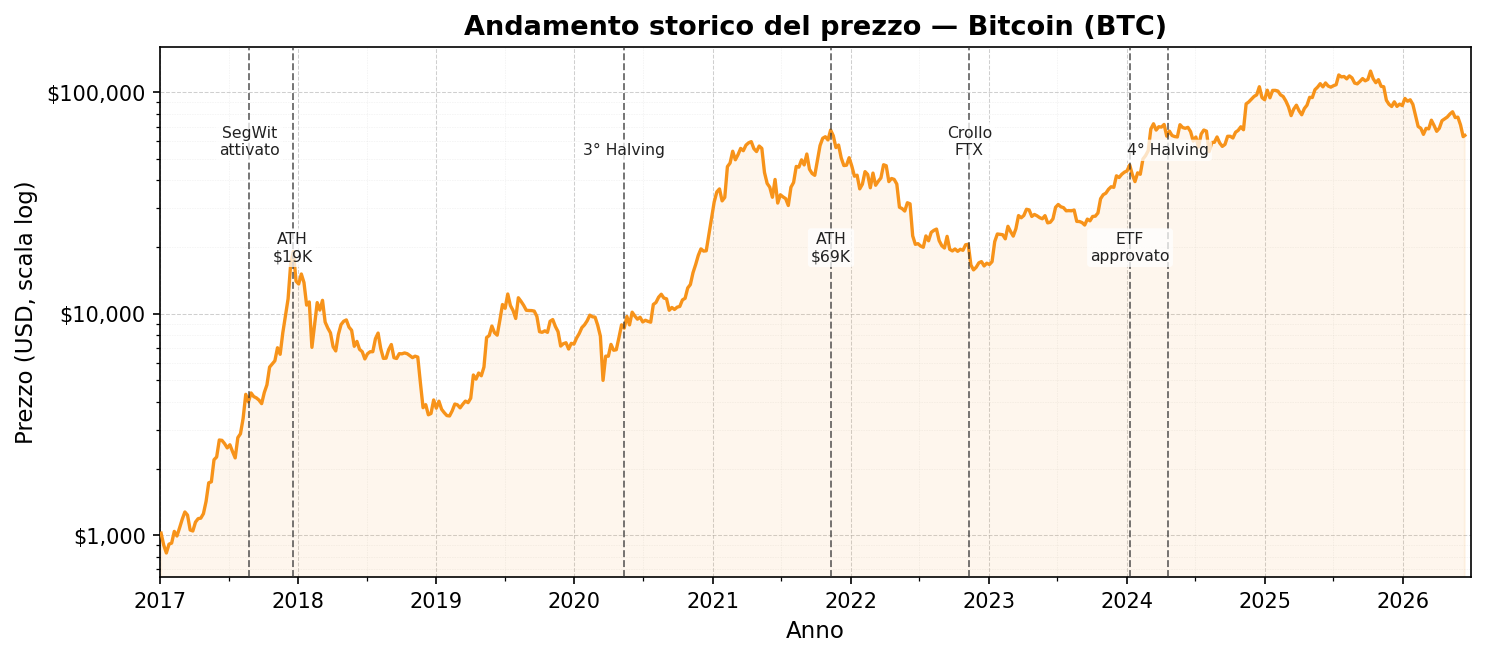
\includegraphics[width=0.90\textwidth]{plots/bitcoin/price_history.png}
    \vspace{0.4em}
    {\small
    \begin{tabular}{@{}ll@{}}
        \toprule
        Data & Evento \\
        \midrule
        Ago.\ 2017 & Attivazione di SegWit \\
        Dic.\ 2017 & ATH a \$19.000 \\
        Mag.\ 2020 & Terzo halving \\
        Nov.\ 2021 & ATH a \$69.000 \\
        Nov.\ 2022 & Crollo FTX \\
        Gen.\ 2024 & Approvazione ETF spot SEC \\
        Apr.\ 2024 & Quarto halving \\
        \bottomrule
    \end{tabular}
    }
    \caption{Andamento storico del prezzo di Bitcoin in USD (2017--2026), scala logaritmica. ATH: All-Time High. Le linee tratteggiate corrispondono agli eventi in tabella. Fonte: CoinMarketCap \cite{CoinMarketCap}.}
    \label{fig:btc_price}
\end{figure}

Come si osserva in Figura~\ref{fig:btc_price}, Bitcoin è l'asset di riferimento dell'intero mercato crypto e il suo storico è scandito da cicli macroeconomici quadriennali legati all'halving. Il termine ATH, All-Time High, indica il massimo storico assoluto raggiunto dal prezzo di un asset. Il primo ATH si colloca nel dicembre 2017 a circa \$19.000, preceduto dall'attivazione di SegWit nell'agosto dello stesso anno, evento che ha reso tecnicamente possibile la Lightning Network. Il successivo mercato ribassista del 2018--2019 precede il terzo halving del maggio 2020, dopodiché il prezzo riprende a salire fino all'ATH di circa \$69.000 nel novembre 2021. Il crollo del novembre 2022, indicato come ``crollo FTX'', coincide con il fallimento dell'omonimo exchange fondato da Samuel Bankman-Fried per gravi irregolarità nella gestione dei fondi dei clienti, innescando un panico di vendite generalizzato sull'intero mercato. La ripresa del 2023--2024 culmina con l'approvazione degli ETF spot Bitcoin da parte della SEC nel gennaio 2024. Un ETF spot (Exchange-Traded Fund) è uno strumento finanziario che detiene direttamente l'asset sottostante e ne replica il prezzo in tempo reale; la sua approvazione ha permesso agli investitori istituzionali di esporsi a Bitcoin attraverso i mercati regolamentati tradizionali senza custodire la criptovaluta. Il quarto halving dell'aprile 2024 ha ulteriormente sostenuto la domanda, portando il prezzo su nuovi massimi nel 2025. La rete Lightning ha vissuto fasi di adozione massiva durante i bull run del 2017, del 2021 e del 2024--2025, intervallate da periodi di consolidamento infrastrutturale durante i mercati ribassisti del 2018 e del 2022.

\subsection{Analisi delle Metriche e Discussione dei Plot}

\subsubsection{Distribuzione dei Gradi e Proprietà Scale-Free}
\begin{figure}[H]
    \centering
    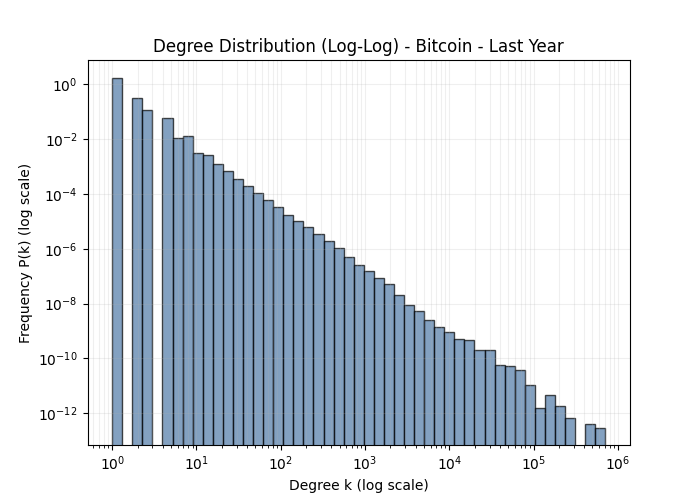
\includegraphics[width=0.65\textwidth]{plots/bitcoin/DegreeDistribution.png}
    \caption{Distribuzione dei gradi $P(k)$ in scala log-log per la rete Lightning di Bitcoin.}
    \label{fig:btc_degree}
\end{figure}
Il grafico in scala log-log (Figura~\ref{fig:btc_degree}) mostra una decadenza lineare netta che si estende su sei ordini di grandezza in ascissa (da $k=1$ a $k \approx 10^6$) e dodici ordini di grandezza in ordinata (da $P \approx 1$ a $P \approx 10^{-13}$). La linearità della decadenza in scala doppiamente logaritmica è la firma formale di una distribuzione a legge di potenza, confermando la natura \textit{scale-free} della rete. La presenza di nodi con oltre un milione di canali attivi indica l'esistenza di operatori commerciali di routing specializzato che concentrano su di sé una quota sproporzionata del traffico di instradamento.

\subsubsection{Average Neighbor Degree ($AND$)}
\begin{figure}[H]
    \centering
    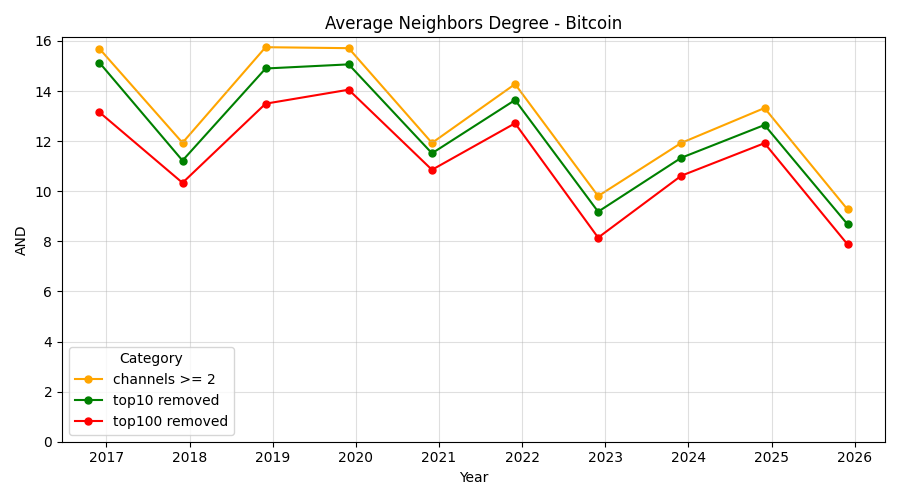
\includegraphics[width=0.65\textwidth]{plots/bitcoin/AverageNeighborsDegree.png}
    \caption{Andamento storico dell'Average Neighbor Degree (AND) per Bitcoin (2017--2026).}
    \label{fig:btc_and}
\end{figure}
Il plot dell'AND (Figura~\ref{fig:btc_and}) rivela un andamento oscillatorio con una periodicità correlata ai cicli macroeconomici di Bitcoin, visibili nel grafico del prezzo (Figura~\ref{fig:btc_price}). Si osservano picchi negli anni 2017 ($\sim$16), 2019--2020 ($\sim$16.5) e 2022 ($\sim$14.3), con minimi in 2018 ($\sim$10.5), 2021 ($\sim$12) e nel minimo assoluto del 2023 ($\sim$8.2 per la curva \texttt{top100 removed}), anno successivo al crollo di FTX. Durante le fasi ribassiste, i nodi periferici con scarsa liquidità chiudono i canali, lasciando un grafo residuo composto da connessioni hub-to-hub che riduce il grado medio percepito dalla periferia. Il gap costante di $\sim$2--3 unità tra curva arancione e rossa conferma la presenza stabile di hub dominanti in ogni snapshot annuale.

\subsubsection{Clustering Coefficient ($CC$)}
\begin{figure}[H]
    \centering
    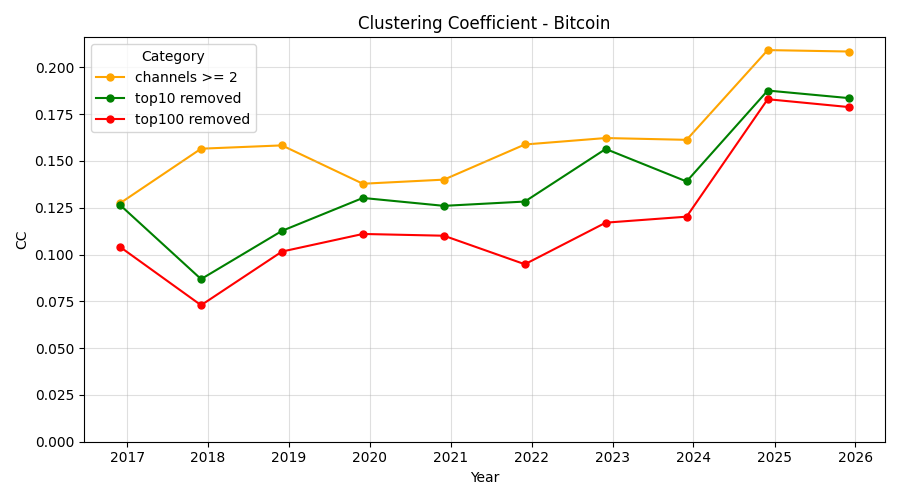
\includegraphics[width=0.65\textwidth]{plots/bitcoin/ClusteringCoefficient.png}
    \caption{Evoluzione del Clustering Coefficient locale e globale in Bitcoin.}
    \label{fig:btc_cc}
\end{figure}
Il CC (Figura~\ref{fig:btc_cc}) mostra valori globalmente contenuti, con un minimo assoluto nel 2018 (curva \texttt{top100 removed}: $\sim$0.073), anno di massima contrazione post-ATH. A partire dal 2023 si osserva un trend incrementale che culmina nel 2025 in un salto significativo: la curva arancione raggiunge $\sim$0.21 e la rossa $\sim$0.183, livelli mai raggiunti nel decennio precedente. Questo aumento coincide con il bull market del 2024--2025 (quarto halving e approvazione degli ETF spot), suggerendo che i nuovi partecipanti formino cluster locali più densi rispetto ai cicli precedenti. La progressiva convergenza delle tre curve dopo il 2024 indica una distribuzione più uniforme della triangolazione locale.

\subsubsection{Network Centralization ($NC$)}
\begin{figure}[H]
    \centering
    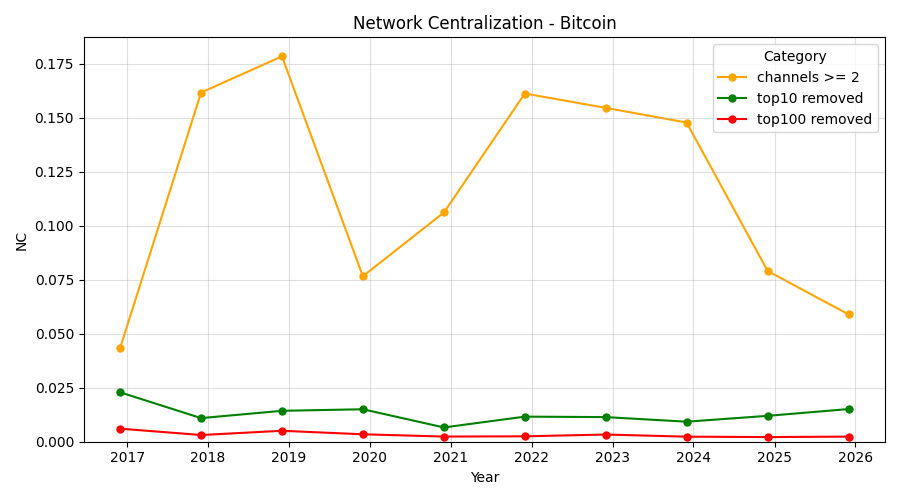
\includegraphics[width=0.65\textwidth]{plots/bitcoin/NetworkCentralization.png}
    \caption{Network Centralization (NC) e polarizzazione globale del grafo in Bitcoin.}
    \label{fig:btc_nc}
\end{figure}
La curva arancione della NC (Figura~\ref{fig:btc_nc}) oscilla tra 0.042 (2017) e 0.178 (2019), con un secondo picco a $\sim$0.161 nel 2022. Un dato controintuitivo ma strutturalmente rilevante è che i picchi di NC si registrano negli anni immediatamente \textit{successivi} ai massimi di prezzo (2019 dopo l'ATH del 2017; 2022 dopo l'ATH del 2021): nelle fasi ribassiste i nodi periferici inattivi escono dal grafo, rendendo gli hub residui proporzionalmente più dominanti. La marcata discesa dopo il 2022, fino a 0.059 nel 2026, segnala una progressiva decentralizzazione organica. Le curve verde e rossa rimangono praticamente a zero per l'intero decennio, confermando che tutta l'asimmetria strutturale è attribuibile a un numero ristrettissimo di hub.

\subsubsection{Componenti Connesse}
\begin{figure}[H]
    \centering
    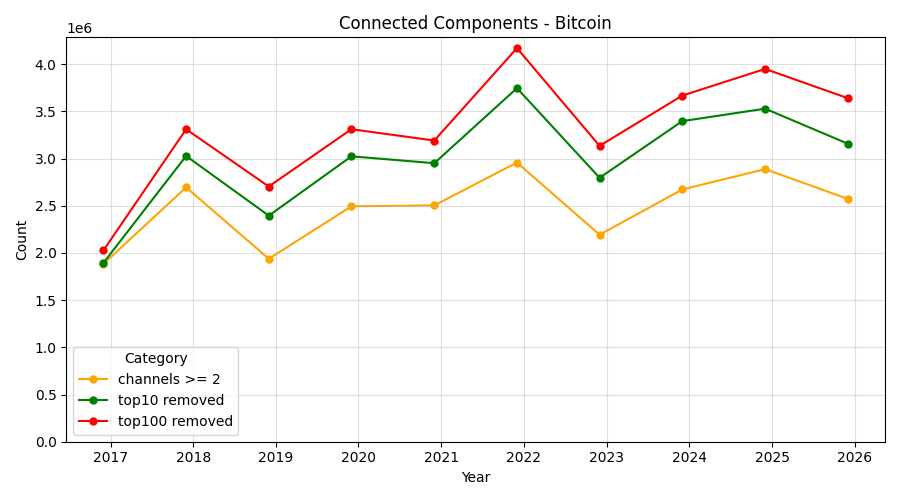
\includegraphics[width=0.65\textwidth]{plots/bitcoin/ConnectedComponents.png}
    \caption{Analisi del numero di componenti connesse e tasso di isolamento in Bitcoin.}
    \label{fig:btc_cc_comp}
\end{figure}
Il grafico delle componenti connesse (Figura~\ref{fig:btc_cc_comp}) rivela che la rete Bitcoin, anche nel caso del grafo completo (curva arancione), presenta tra 1.9 e 3 milioni di componenti connesse distinte. La rete non è una struttura monolitica ma un nucleo di routing centrale circondato da milioni di piccoli subgraph isolati, tipicamente coppie bilaterali di nodi con canali tra loro non connesse al routing principale. Rimuovendo i 100 hub principali (curva rossa), il conteggio sale fino a 4.2 milioni nel picco del 2022, evidenziando il ruolo critico degli hub come ponte tra il nucleo di routing e i subgraph periferici. Il crescente divario tra curva arancione e rossa nel tempo indica che la dipendenza dalla mediazione degli hub è aumentata nel corso del decennio. È importante notare che questo elevato numero di componenti non è in contraddizione con i valori di AND ($\sim$8--16) riportati nella sezione precedente: l'AND viene calcolato sui soli nodi con almeno un vicino nel grafo filtrato, ovvero il nucleo di routing attivo, mentre il conteggio delle componenti include tutti i nodi mai osservati, compresi quelli delle coppie isolate inattive. Si tratta di due popolazioni distinte dello stesso grafo.

\subsubsection{Betweenness Centrality ($BC$)}
\begin{figure}[H]
    \centering
    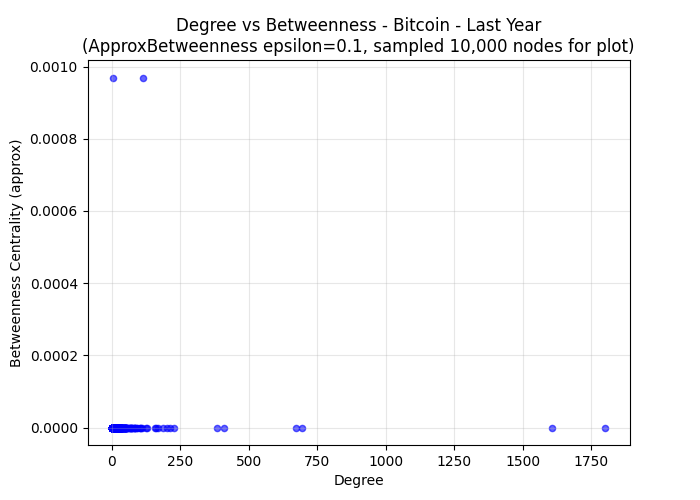
\includegraphics[width=0.65\textwidth]{plots/bitcoin/NodeDegreeBetweennessCentrality.png}
    \caption{Relazione tra Degree e Betweenness Centrality in Bitcoin.}
    \label{fig:btc_bc}
\end{figure}
Il plot Degree-Betweenness (Figura~\ref{fig:btc_bc}) mostra che la quasi totalità dei nodi si posiziona su valori di BC prossimi allo zero, indipendentemente dal grado. Il dato più rilevante è la presenza di un nodo con grado basso ($k \approx 10$--$20$) e BC di $\sim$0.00096, il valore più alto dell'intero campione, superiore persino a quello dell'hub principale (grado $\sim$3000, BC $\approx 0$). Questo nodo è classificabile come \textit{bridge node}: pur possedendo pochissimi canali, occupa una posizione topologica critica che lo rende l'unico percorso minimo tra due grandi porzioni della rete, conferendogli un potere di intermediazione sproporzionato rispetto alla sua connettività apparente.

\subsubsection{Small World Check}
\begin{figure}[H]
    \centering
    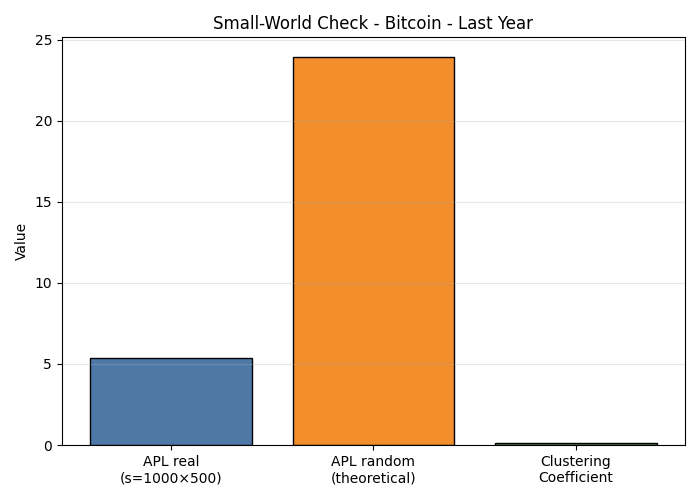
\includegraphics[width=0.65\textwidth]{plots/bitcoin/SmallWorld.png}
    \caption{Verifica Small World: APL reale vs.\ modello casuale in Bitcoin.}
    \label{fig:btc_sw}
\end{figure}
Il grafico a barre (Figura~\ref{fig:btc_sw}) formalizza la proprietà Small World della rete Lightning di Bitcoin. L'APL reale si attesta a $\sim$5.35 salti medi, a fronte di un valore teorico atteso per un grafo casuale di pari dimensioni pari a $\sim$24. Il rapporto di efficienza ($\sim$4.5$\times$) indica che la rete minimizza strutturalmente la lunghezza dei percorsi di pagamento. Il Clustering Coefficient ($\sim$0.21) completa la verifica: la rete Bitcoin soddisfa pienamente entrambe le condizioni del modello Watts-Strogatz.

\subsection{Conclusioni e Comparazione}
La rete Lightning di Bitcoin esibisce la topologia più matura e strutturalmente stabile del pannello analizzato. Il pattern oscillatorio dell'AND, direttamente correlabile ai cicli di halving quadriennale osservabili nel grafico del prezzo, dimostra come la struttura topologica risponda in modo sistematico alle dinamiche macroeconomiche dell'asset sottostante. Il progressivo abbassamento della Network Centralization dopo il 2022, combinato con l'aumento del Clustering Coefficient nel 2024--2025, suggerisce una tendenza verso una distribuzione più diffusa della connettività, pur restando la struttura hub-and-spoke il meccanismo dominante di routing. La presenza di un bridge node ad alta BC e basso grado rappresenta un punto di fragilità strutturale non rilevabile attraverso l'analisi dei soli hub principali.

\newpage

\section{Risultati Relativi a Ethereum (ETH)}
Questo capitolo presenta i risultati dell'analisi topologica per la rete di canali di Ethereum (Raiden Network), calcolati sugli snapshot annuali 2017--2026 con la metodologia descritta nel Capitolo~2.

\subsection{Introduzione Storica}

\begin{figure}[H]
    \centering
    
\includegraphics[width=0.90\textwidth]{plots/ethereum/price_history.png}
    \vspace{0.4em}
    {\small
    \begin{tabular}{@{}ll@{}}
        \toprule
        Data & Evento \\
        \midrule
        Gen.\ 2018 & ATH a \$1.400 \\
        Lug.\ 2020 & DeFi Summer \\
        Nov.\ 2021 & ATH a \$4.900 \\
        Set.\ 2022 & The Merge (transizione a Proof-of-Stake) \\
        Nov.\ 2022 & Crollo FTX \\
        \bottomrule
    \end{tabular}
    }
    \caption{Andamento storico del prezzo di Ethereum in USD (2017--2026), scala logaritmica. Le linee tratteggiate corrispondono agli eventi in tabella. Fonte: CoinMarketCap \cite{CoinMarketCap}.}
    \label{fig:eth_price}
\end{figure}

Come si osserva in Figura~\ref{fig:eth_price}, Ethereum mostra una dinamica di prezzo distinta rispetto a Bitcoin. Il primo ATH si registra nel gennaio 2018 a $\sim$\$1.400, seguito da un mercato ribassista protratto fino al 2019. La DeFi Summer del luglio 2020 ha segnato la ripresa: lo sviluppo dei canali di pagamento off-chain, tra cui la Raiden Network, ha vissuto il suo momento di massimo interesse nel biennio 2020--2021, e l'esplosione dell'attività DeFi ha portato l'ecosistema al secondo ATH di $\sim$\$4.900 nel novembre 2021.

Il settembre 2022 è segnato da The Merge, l'evento con cui Ethereum ha completato la transizione dal meccanismo di consenso Proof-of-Work al Proof-of-Stake. Nel Proof-of-Work i partecipanti competono risolvendo problemi computazionali complessi per validare i blocchi; nel Proof-of-Stake la validazione è affidata a chi deposita in garanzia una quota di criptovaluta, eliminando il consumo energetico del mining. The Merge non ha interrotto la fase ribassista già in corso, aggravata nel novembre 2022 dal crollo di FTX. A partire dal 2022 la roadmap ufficiale di Ethereum si è spostata verso i rollup come soluzione di scaling preferita, marginalizzando progressivamente la Raiden Network e i canali di pagamento puri. Dal 2023 il prezzo riprende a salire, con una traiettoria meno accentuata rispetto a Bitcoin.

\subsection{Analisi delle Metriche e Discussione dei Plot}

\subsubsection{Distribuzione dei Gradi e Topologia}
\begin{figure}[H]
    \centering
    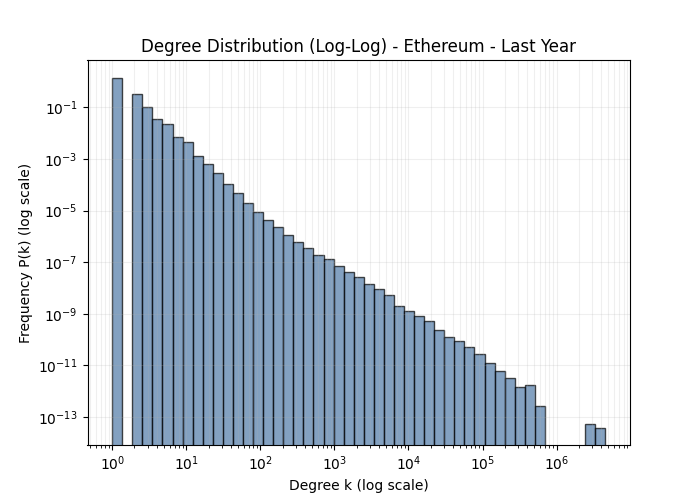
\includegraphics[width=0.65\textwidth]{plots/ethereum/DegreeDistribution.png}
    \caption{Distribuzione dei gradi $P(k)$ in scala log-log per l'infrastruttura canali di Ethereum.}
    \label{fig:eth_degree}
\end{figure}
La Figura~\ref{fig:eth_degree} mostra una decadenza log-log lineare coerente con la natura scale-free della rete, con la coda che si estende fino a $k \approx 1750$: quattro ordini di grandezza inferiore rispetto a Bitcoin, riflettendo la dimensione complessivamente più contenuta del network Raiden. La pendenza della distribuzione è comparabile a quella delle reti Lightning analizzate, confermando che la concentrazione del grado attorno agli hub segue la medesima legge di potenza. La separazione verticale tra le tre curve (\texttt{channels $\ge$ 2}, \texttt{top10 removed}, \texttt{top100 removed}) è meno pronunciata rispetto a Bitcoin, suggerendo che il contributo strutturale degli hub sia proporzionalmente meno dominante, pur mantenendo la stessa topologia scale-free.

\subsubsection{Average Neighbor Degree ($AND$)}
\begin{figure}[H]
    \centering
    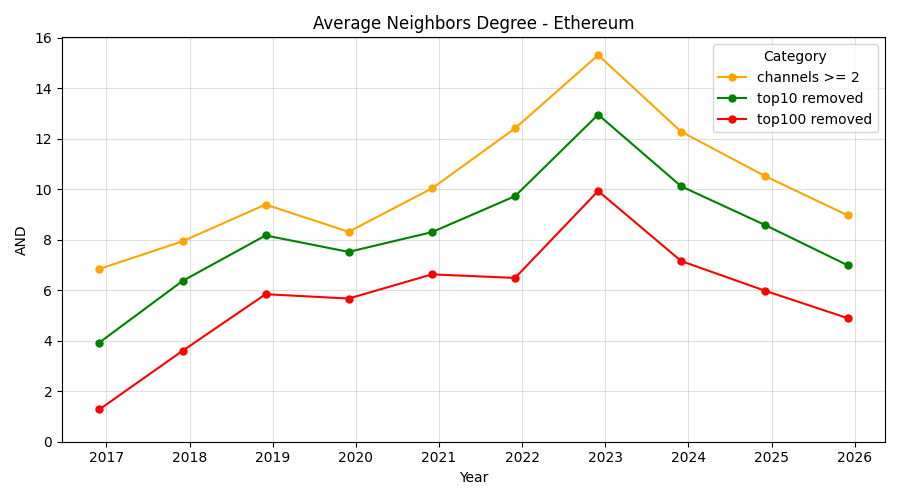
\includegraphics[width=0.65\textwidth]{plots/ethereum/AverageNeighborsDegree.png}
    \caption{Evoluzione temporale dell'Average Neighbor Degree (AND) in Ethereum.}
    \label{fig:eth_and}
\end{figure}
L'AND di Ethereum (Figura~\ref{fig:eth_and}) mostra un andamento monotonicamente crescente da $\sim$6.8 nel 2017 fino a un picco di $\sim$15.3 nel 2023, seguito da un calo a $\sim$9 nel 2026. Questo profilo differisce strutturalmente dall'oscillazione ciclica osservata in Bitcoin: la crescita monotonica riflette l'espansione progressiva dell'ecosistema DeFi (visibile come DeFi Summer nel grafico del prezzo, Figura~\ref{fig:eth_price}) e la conseguente attrazione di nodi con connettività elevata. Il calo post-2023, correlabile alla progressiva migrazione dell'ecosistema verso i rollup come soluzione di scaling preferita, indica una riduzione della centralità percepita dai nodi periferici a favore di una struttura più stratificata.

\subsubsection{Clustering Coefficient ($CC$)}
\begin{figure}[H]
    \centering
    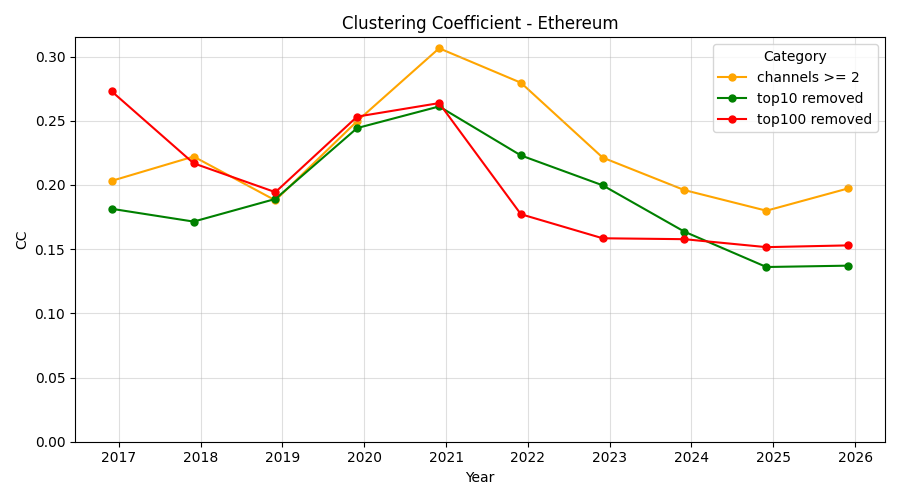
\includegraphics[width=0.65\textwidth]{plots/ethereum/ClusteringCoefficient.png}
    \caption{Andamento storico del Clustering Coefficient (CC) in Ethereum.}
    \label{fig:eth_cc}
\end{figure}
Il CC di Ethereum (Figura~\ref{fig:eth_cc}) presenta un'anomalia degna di nota nel 2017: la curva rossa (\texttt{top100 removed}) supera quella arancione (\texttt{channels $\ge$ 2}), attestandosi rispettivamente a $\sim$0.274 contro $\sim$0.204. In tutte le altre reti e in tutti gli altri anni il rapporto è invertito. Questo fenomeno indica che nel 2017, data la dimensione ancora ridotta del network, i 100 nodi principali abbassavano il CC medio agendo come hub di transito poco triangolati; rimuoverli aumentava il clustering del grafo residuo. Il picco assoluto si registra nel 2021 ($\sim$0.308 sulla curva arancione), coincidendo con l'ATH di prezzo e l'esplosione dell'attività DeFi. Il valore scende poi progressivamente fino a $\sim$0.22 nel 2026.

\subsubsection{Network Centralization ($NC$)}
\begin{figure}[H]
    \centering
    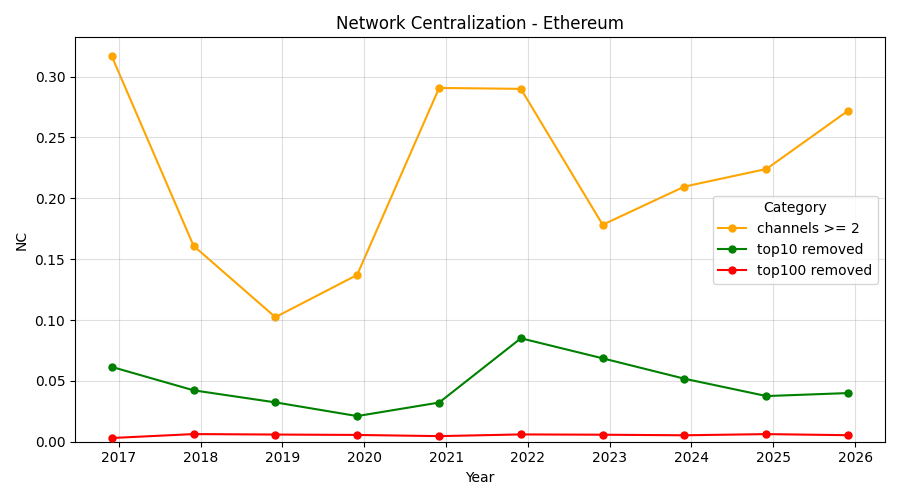
\includegraphics[width=0.65\textwidth]{plots/ethereum/NetworkCentralization.png}
    \caption{Network Centralization e varianza dell'indice di polarizzazione in Ethereum.}
    \label{fig:eth_nc}
\end{figure}
Ethereum presenta i valori di NC più elevati tra tutte le reti del pannello (Figura~\ref{fig:eth_nc}). La curva arancione parte da $\sim$0.315 nel 2017, rimane elevata a $\sim$0.292 nel biennio 2021--2022 e non scende sotto $\sim$0.274 nemmeno nel 2026. Questa centralizzazione strutturale persistente suggerisce che il network Raiden/Ethereum non ha mai sviluppato la stessa varietà di operatori di routing intermedi osservata in Bitcoin e Litecoin: pochi nodi dominano l'intera topologia in modo stabile nel tempo, indipendentemente dalle fasi di mercato.

\subsubsection{Componenti Connesse}
\begin{figure}[H]
    \centering
    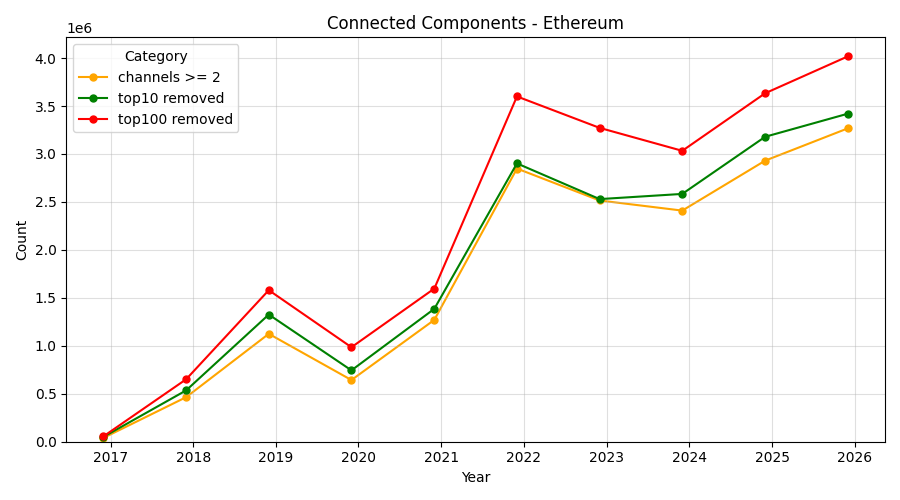
\includegraphics[width=0.65\textwidth]{plots/ethereum/ConnectedComponents.png}
    \caption{Evoluzione delle componenti connesse in Ethereum.}
    \label{fig:eth_cc_comp}
\end{figure}
Il grafico delle componenti connesse (Figura~\ref{fig:eth_cc_comp}) rivela una dinamica radicalmente diversa rispetto a Bitcoin e Litecoin. Il numero di componenti è quasi nullo nel 2017, cresce gradualmente e raggiunge 3.3--4 milioni nel 2026. Le tre curve sono quasi perfettamente sovrapposte per l'intero arco temporale: rimuovere i 100 hub principali non altera significativamente il conteggio delle componenti. Questo indica che la frammentazione della rete Ethereum è un fenomeno intrinseco della struttura dei canali e non dipende dagli hub, a differenza di Bitcoin dove i top-100 svolgono un ruolo attivo di raccordo tra subgraph isolati. Va tuttavia segnalata un'osservazione critica: il network Raiden su Ethereum è storicamente più piccolo di Bitcoin Lightning in termini di nodi attivi di routing, eppure raggiunge un conteggio di componenti comparabile. Questo suggerisce che i dati BigQuery catturano l'intero universo dei payment channel contract mai deployati su Ethereum, inclusi canali one-shot di protocolli DeFi, state channel sperimentali e canali mai entrati nel routing principale: la stragrande maggioranza delle componenti è quindi costituita da subgraph storici inattivi, non da nodi correntemente operativi.

\subsubsection{Betweenness Centrality ($BC$)}
\begin{figure}[H]
    \centering
    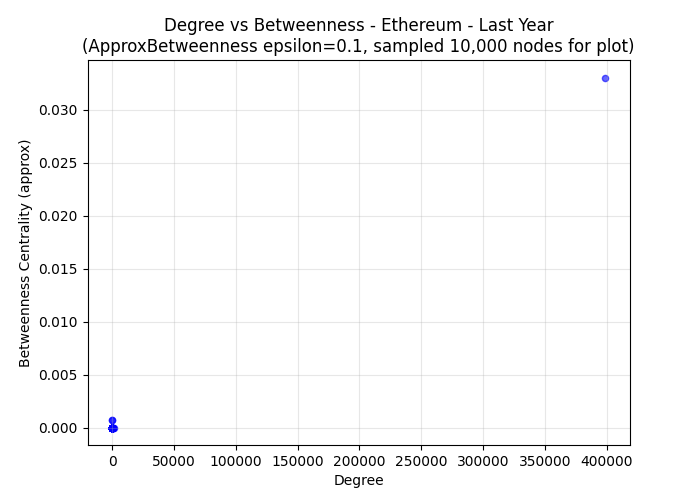
\includegraphics[width=0.65\textwidth]{plots/ethereum/NodeDegreeBetweennessCentrality.png}
    \caption{Distribuzione della Betweenness Centrality in funzione del grado in Ethereum.}
    \label{fig:eth_bc}
\end{figure}
Il plot Degree-Betweenness di Ethereum (Figura~\ref{fig:eth_bc}) mostra una caratteristica assente nelle altre reti: la presenza di valori di BC \textit{negativi}. Poiché la BC per definizione non può essere negativa, questi valori sono un artefatto dell'approssimazione stocastica di NetworKit con parametri $\varepsilon = 0.1$, $\delta = 0.1$ applicata a una rete di dimensioni relativamente contenute. Il grado massimo osservato è $k \approx 1750$, sensibilmente inferiore ai picchi di Bitcoin ($k \approx 10^6$), confermando la minore espansione orizzontale del network.

\subsubsection{Small World Check}
\begin{figure}[H]
    \centering
    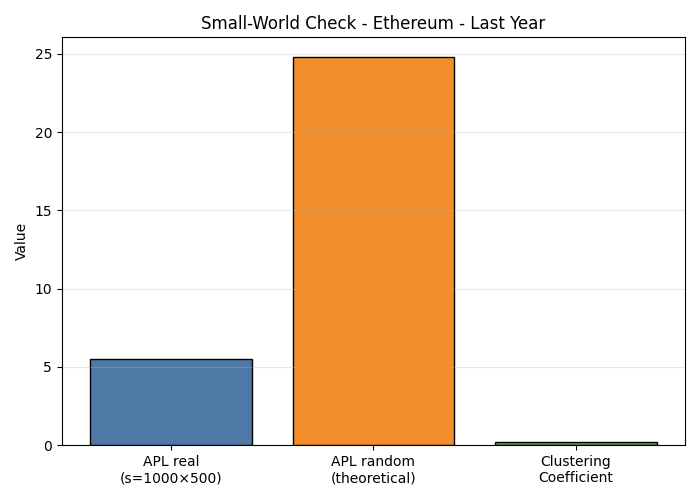
\includegraphics[width=0.65\textwidth]{plots/ethereum/SmallWorld.png}
    \caption{Rapporto di efficienza APL e validazione Small World in Ethereum.}
    \label{fig:eth_sw}
\end{figure}
Il grafico a barre (Figura~\ref{fig:eth_sw}) mostra che Ethereum raggiunge l'APL reale più basso tra tutte le reti analizzate: $\sim$4.3 salti contro un valore atteso per un grafo casuale di $\sim$24.8. Questo risultato, apparentemente paradossale per una rete meno grande, è spiegabile dall'elevata NC: una struttura fortemente centralizzata riduce geometricamente le distanze medie poiché quasi ogni percorso passa attraverso un numero ristretto di hub principali, accorciando i cammini minimi a scapito della resilienza.

\subsection{Conclusioni e Comparazione}
La rete di canali di Ethereum si distingue per una centralizzazione strutturale persistente e storicamente la più elevata del pannello, con valori di NC mai scesi sotto $\sim$0.27 in un decennio. L'anomalia del 2017 nel Clustering Coefficient e la presenza di valori di BC negativi, artefatto dell'approssimazione stocastica su una rete di piccole dimensioni, testimoniano le specificità di una rete che non ha raggiunto la maturità topologica di Bitcoin. L'APL più basso del campione ($\sim$4.3) è una conseguenza diretta della centralizzazione, non un indicatore di robustezza distribuita: una rete che instrada quasi tutto il traffico attraverso pochi hub è efficiente per definizione, ma vulnerabile in misura proporzionale.

\newpage

\section{Risultati Relativi a Litecoin (LTC)}
Questo capitolo presenta i risultati dell'analisi topologica per la rete Lightning di Litecoin, calcolati sugli snapshot annuali 2017--2026 con la metodologia descritta nel Capitolo~2.

\subsection{Introduzione Storica}

\begin{figure}[H]
    \centering
    
\includegraphics[width=0.90\textwidth]{plots/litecoin/price_history.png}
    \vspace{0.4em}
    {\small
    \begin{tabular}{@{}ll@{}}
        \toprule
        Data & Evento \\
        \midrule
        Mag.\ 2017 & Attivazione di SegWit su Litecoin \\
        Dic.\ 2017 & ATH a \$375 \\
        Ago.\ 2019 & Terzo halving \\
        Nov.\ 2022 & Crollo FTX \\
        Ago.\ 2023 & Quarto halving \\
        \bottomrule
    \end{tabular}
    }
    \caption{Andamento storico del prezzo di Litecoin in USD (2017--2026), scala logaritmica. Le linee tratteggiate corrispondono agli eventi in tabella. Fonte: CoinMarketCap \cite{CoinMarketCap}.}
    \label{fig:ltc_price}
\end{figure}

Come si osserva in Figura~\ref{fig:ltc_price}, Litecoin evidenzia una struttura ciclica analoga a quella di Bitcoin, ma con ampiezze di oscillazione inferiori. Lanciato nel 2011 come fork del codice core di Bitcoin con architettura UTXO, ha anticipato Bitcoin nell'adozione di SegWit nel maggio 2017, diventando il terreno di prova ideale per le prime implementazioni della Lightning Network. L'attivazione di SegWit coincide con il primo rialzo significativo dell'anno, che culmina nell'ATH del dicembre 2017 a $\sim$\$375. Il terzo halving dell'agosto 2019 si colloca in un momento di mercato laterale e non produce un immediato rimbalzo del prezzo, a differenza di Bitcoin. Il picco del 2021 risulta meno pronunciato rispetto agli altri asset del pannello, confermando la progressiva perdita di quota di mercato di Litecoin. Il crollo di FTX del novembre 2022 ha colpito anche Litecoin, trascinandone il prezzo al ribasso. La flessione è seguita da una ripresa graduale nel 2023, anno in cui si colloca anche il quarto halving di agosto. Lo sviluppo della rete off-chain ha registrato una crescita progressiva e lineare, con picchi di capillarità operativa tra il 2025 e il 2026.

\subsection{Analisi delle Metriche e Discussione dei Plot}

\subsubsection{Distribuzione dei Gradi}
\begin{figure}[H]
    \centering
    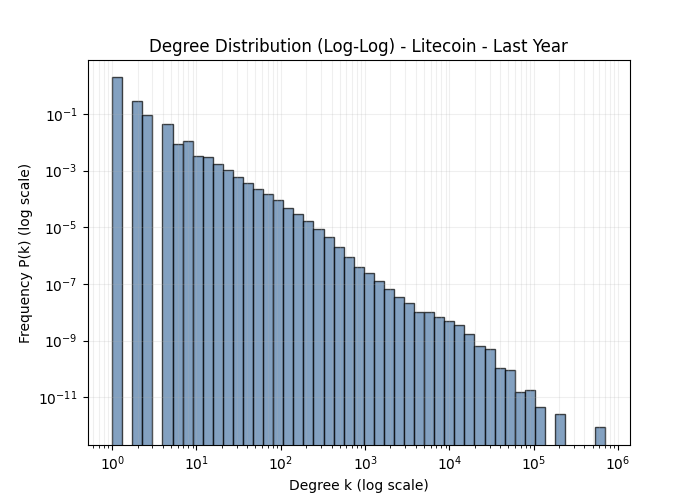
\includegraphics[width=0.65\textwidth]{plots/litecoin/DegreeDistribution.png}
    \caption{Distribuzione dei gradi $P(k)$ in scala log-log per la rete Lightning di Litecoin.}
    \label{fig:ltc_degree}
\end{figure}
Il plot log-log di Litecoin (Figura~\ref{fig:ltc_degree}) replica fedelmente la pendenza e l'estensione della distribuzione scale-free osservata in Bitcoin, con la coda che si estende fino a $k \approx 10^6$ e la stessa decadenza lineare su sei ordini di grandezza. Il parallelismo è più stretto rispetto a qualsiasi altra coppia di reti nel pannello, ed è l'esito diretto della condivisione della medesima codebase di Lightning Network e della struttura UTXO con SegWit.

\subsubsection{Average Neighbor Degree ($AND$)}
\begin{figure}[H]
    \centering
    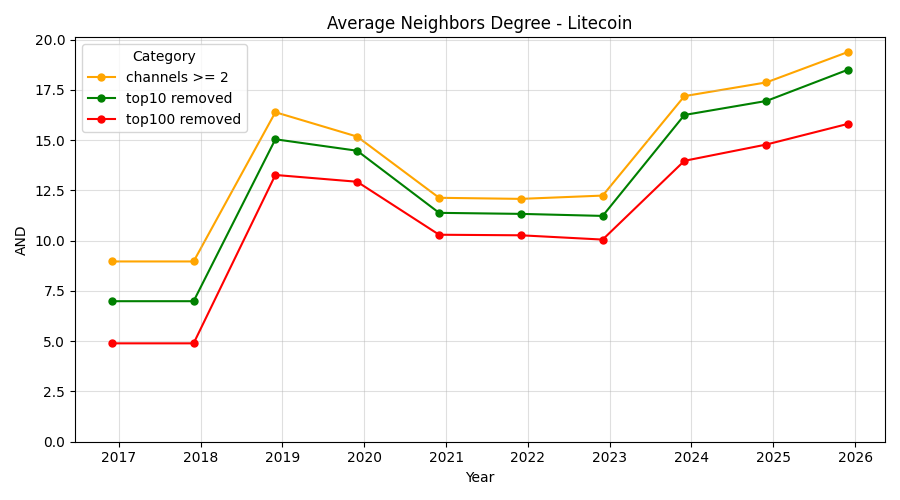
\includegraphics[width=0.65\textwidth]{plots/litecoin/AverageNeighborsDegree.png}
    \caption{Trend di crescita dell'Average Neighbor Degree (AND) in Litecoin.}
    \label{fig:ltc_and}
\end{figure}
L'AND di Litecoin (Figura~\ref{fig:ltc_and}) presenta il profilo più caratteristico del pannello: pressoché costante a $\sim$9 nel biennio 2017--2018, subisce un salto brusco nel 2019 portandosi a $\sim$16.5, e poi riprende una crescita monotonica fino a $\sim$19.3 nel 2026. Il 2019 coincide con il terzo halving (agosto 2019, visibile nel grafico del prezzo, Figura~\ref{fig:ltc_price}): il taglio del premio attirò un'ondata di nodi di routing professionali che aumentarono la connettività percepita dalla periferia in modo discontinuo. Il gap arancione-rosso, moderato nel periodo 2017--2018, si allarga dopo il 2019 ($\sim$3--4 unità), confermando che i nuovi hub post-halving erano più connessi della media.

\subsubsection{Clustering Coefficient ($CC$)}
\begin{figure}[H]
    \centering
    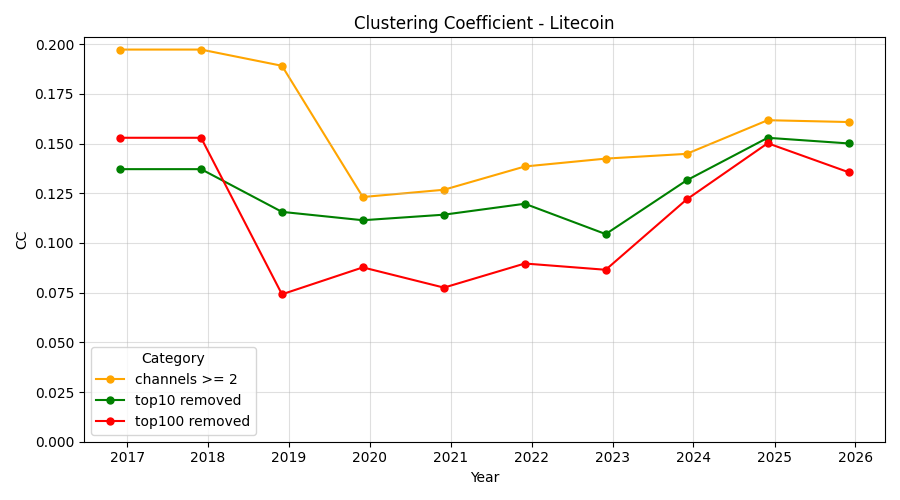
\includegraphics[width=0.65\textwidth]{plots/litecoin/ClusteringCoefficient.png}
    \caption{Clustering Coefficient e analisi della ridondanza locale in Litecoin.}
    \label{fig:ltc_cc}
\end{figure}
Il CC di Litecoin (Figura~\ref{fig:ltc_cc}) mostra un comportamento \textit{inverso} rispetto all'AND: il valore arancione parte da $\sim$0.197 nel 2017, poi cala bruscamente al minimo di $\sim$0.075 nel 2019 (la curva rossa scende ancora di più), per risalire gradualmente fino a $\sim$0.130 nel 2026. La discesa del 2019 è la controparte geometrica del salto dell'AND: l'ingresso massiccio di hub molto connessi abbassa il clustering medio perché questi hub fungono da stella-centro senza formare triangoli con i vicini. L'inversione di tendenza post-2019 riflette la progressiva maturazione del network con la formazione di ridondanze locali tra i routing node.

\subsubsection{Network Centralization ($NC$)}
\begin{figure}[H]
    \centering
    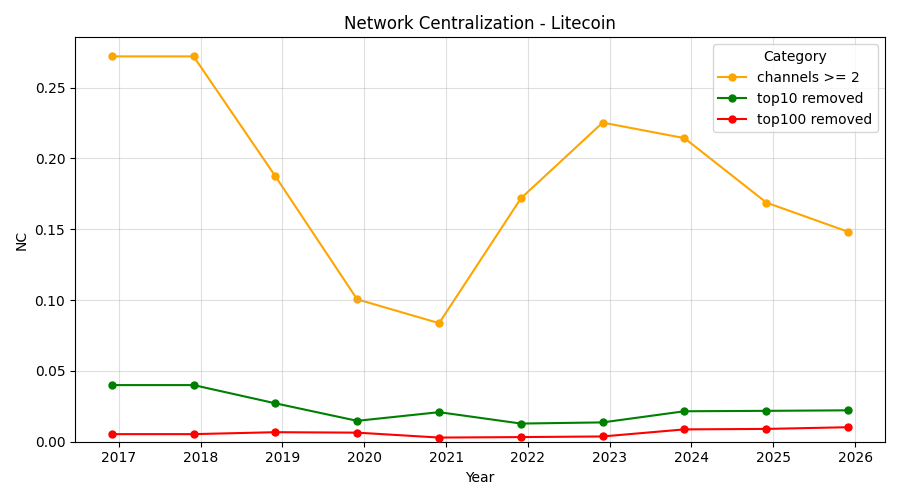
\includegraphics[width=0.65\textwidth]{plots/litecoin/NetworkCentralization.png}
    \caption{Indice di Network Centralization (NC) nel grafo di Litecoin.}
    \label{fig:ltc_nc}
\end{figure}
La NC di Litecoin (Figura~\ref{fig:ltc_nc}) segue un arco più articolato rispetto a Bitcoin. La curva arancione parte da $\sim$0.270 nel 2017, scende al minimo storico di $\sim$0.083 nel 2021 (massima decentralizzazione relativa, coincidente con il picco di partecipazione al mercato), risale al picco secondario di $\sim$0.226 nel 2023 e si riposiziona a $\sim$0.148 nel 2026. Questo ciclo suggerisce un fenomeno di ri-centralizzazione post-bear market: al calare dei nodi periferici inattivi, gli hub di routing rimasti acquistano proporzionalmente più peso strutturale, senza che il loro numero assoluto sia variato.

\subsubsection{Componenti Connesse}
\begin{figure}[H]
    \centering
    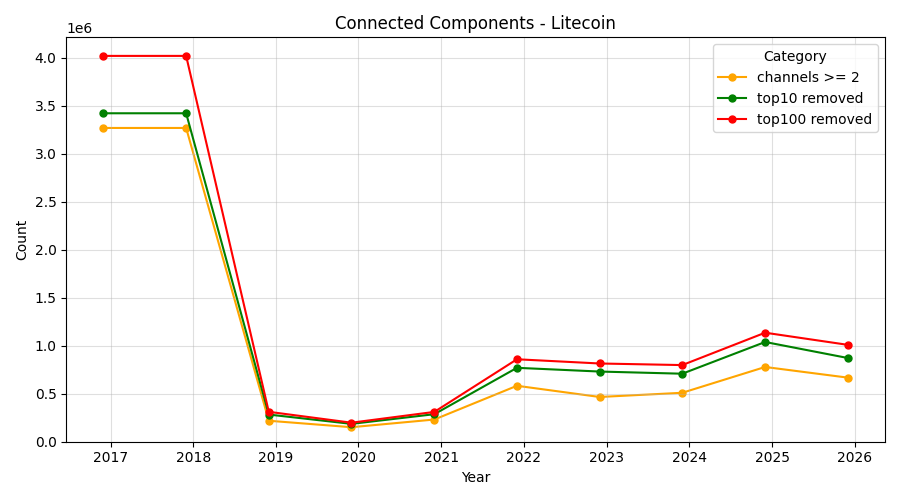
\includegraphics[width=0.65\textwidth]{plots/litecoin/ConnectedComponents.png}
    \caption{Evoluzione delle componenti connesse e collasso strutturale in Litecoin.}
    \label{fig:ltc_cc_comp}
\end{figure}
Il grafico delle componenti connesse (Figura~\ref{fig:ltc_cc_comp}) rivela il fenomeno più drammatico del pannello. Nei primi due anni di snapshot (2017--2018) il numero di componenti si attesta intorno a 3.4 milioni. Nel 2019 cala bruscamente a $\sim$300.000, una riduzione di circa il 91\% in un solo anno. Tutte e tre le curve (\texttt{channels $\ge$ 2}, \texttt{top10 removed}, \texttt{top100 removed}) scendono quasi perfettamente in parallelo, indicando che il collasso non dipende dagli hub ma è un fenomeno strutturale della rete. L'interpretazione più coerente è che nel 2018 un gran numero di nodi isolati sperimentali venne dismesso contestualmente, mentre nel 2019 il halving ridisegnò la composizione del network attivo. Il dato rimane tra 300.000 e 400.000 componenti per tutti gli anni successivi.

\subsubsection{Betweenness Centrality ($BC$)}
\begin{figure}[H]
    \centering
    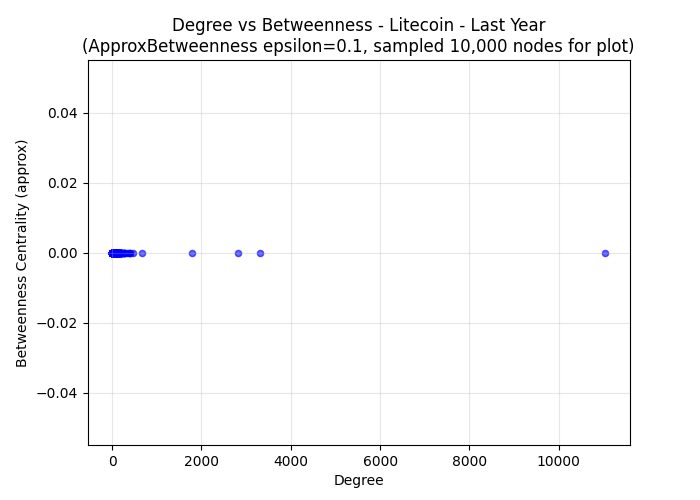
\includegraphics[width=0.65\textwidth]{plots/litecoin/NodeDegreeBetweennessCentrality.png}
    \caption{Profilo di Betweenness Centrality nel network di Litecoin.}
    \label{fig:ltc_bc}
\end{figure}
Il plot Degree-Betweenness di Litecoin (Figura~\ref{fig:ltc_bc}) mostra un pattern analogo a Bitcoin: la massa dei nodi si concentra con BC prossima a zero, mentre il nodo con grado massimo ($k \approx 2800$) raggiunge i valori di BC più elevati. A differenza di Bitcoin, non si osserva un bridge node con grado basso e BC anomalmente alta: in Litecoin la BC è distribuita più regolarmente tra i nodi ad alto grado, senza outlier di posizione topologica critica.

\subsubsection{Small World Check}
\begin{figure}[H]
    \centering
    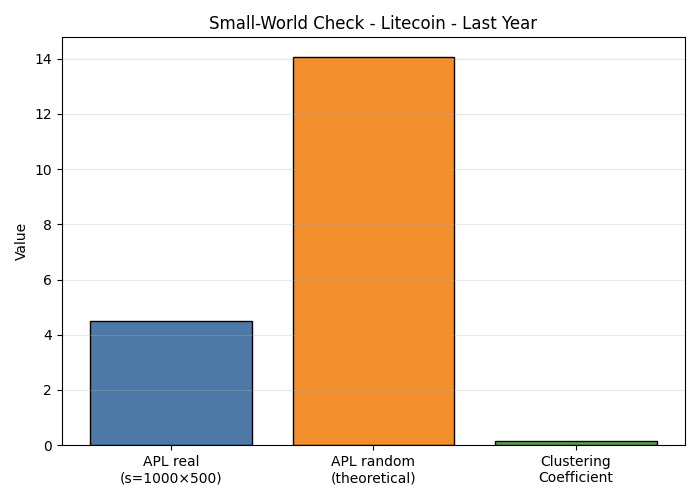
\includegraphics[width=0.65\textwidth]{plots/litecoin/SmallWorld.png}
    \caption{Validazione Small World per Litecoin: APL reale vs.\ modello casuale.}
    \label{fig:ltc_sw}
\end{figure}
Il grafico a barre (Figura~\ref{fig:ltc_sw}) mostra che l'APL reale di Litecoin si attesta a $\sim$4.5 salti, a fronte di un valore atteso per un grafo casuale di $\sim$14.0. Il rapporto di efficienza ($\sim$3.1$\times$) è il più basso del pannello, ma la piccola dimensione assoluta del network giustifica un valore casuale di riferimento già più contenuto. La proprietà Small World è confermata, con il Clustering Coefficient nella barra ($\sim$0.13) che soddisfa la seconda condizione di Watts-Strogatz.

\subsection{Conclusioni e Comparazione}
La rete Lightning di Litecoin presenta la transizione strutturale più netta del pannello: il collasso del 91\% delle componenti connesse nel 2019 e il simultaneo salto dell'AND testimoniano come l'evento del halving abbia operato come un evento di selezione, eliminando i nodi sperimentali e riconfigurando la topologia attorno a operatori di routing professionali. Il parallelismo quasi perfetto con la distribuzione di gradi di Bitcoin conferma la comunanza architetturale, mentre la dinamica di NC e CC rivela cicli di centralizzazione e decentralizzazione correlati ai cicli economici dell'asset sottostante, visibili nel grafico del prezzo (Figura~\ref{fig:ltc_price}).

\newpage

\section{Risultati Relativi a Dogecoin (DOGE)}
Questo capitolo presenta i risultati dell'analisi topologica per il network sperimentale di canali di Dogecoin, calcolati sugli snapshot annuali 2017--2025 con la metodologia descritta nel Capitolo~2.

\subsection{Introduzione Storica}

\begin{figure}[H]
    \centering
    
\includegraphics[width=0.90\textwidth]{plots/dogecoin/price_history.png}
    \vspace{0.4em}
    {\small
    \begin{tabular}{@{}ll@{}}
        \toprule
        Data & Evento \\
        \midrule
        Feb.\ 2021 & Tweet di Elon Musk \\
        Mag.\ 2021 & ATH a \$0.73 \\
        Nov.\ 2022 & Crollo FTX \\
        Apr.\ 2023 & Rebranding Twitter in X \\
        Nov.\ 2024 & Elezioni presidenziali USA \\
        \bottomrule
    \end{tabular}
    }
    \caption{Andamento storico del prezzo di Dogecoin in USD (2017--2025), scala logaritmica. Le linee tratteggiate corrispondono agli eventi in tabella. Fonte: CoinMarketCap \cite{CoinMarketCap}.}
    \label{fig:doge_price}
\end{figure}

Come si osserva in Figura~\ref{fig:doge_price}, Dogecoin presenta una storia di mercato segnata da cicli di volatilità estrema. Nato nel 2013 come criptovaluta ironica derivata da Luckycoin, ha acquisito una rilevanza finanziaria straordinaria trainata da spinte speculative. Sotto il profilo tecnologico, i canali di pagamento Layer 2 su Dogecoin rappresentano un caso di studio limite a causa dei tempi di blocco di 1 minuto e dell'assenza di un supporto SegWit nativo strutturato in modo identico a Bitcoin. Il prezzo di Dogecoin è dominato dall'impennata speculativa del 2021, innescata da una serie di tweet di Elon Musk a partire dal febbraio di quell'anno, e culminata nell'ATH del maggio 2021 a $\sim$\$0.73, circa 150 volte il prezzo di inizio anno. Il crollo successivo è altrettanto rapido, riportando il prezzo a $\sim$\$0.06--0.10 nel corso del 2022, ulteriormente compresso dal crollo di FTX del novembre 2022. Nel 2023 si osserva un nuovo picco di minor entità in corrispondenza del rebranding della piattaforma social Twitter in X, operato da Elon Musk, con cui Dogecoin è storicamente associato per le dichiarazioni pubbliche dello stesso. L'evento più rilevante per il 2024--2025 è il picco successivo alle elezioni presidenziali USA del novembre 2024, con Dogecoin che triplica di valore in poche settimane per poi assestarsi su livelli intermedi nel 2025.

\subsection{Analisi delle Metriche e Discussione dei Plot}

\subsubsection{Distribuzione dei Gradi}
\begin{figure}[H]
    \centering
    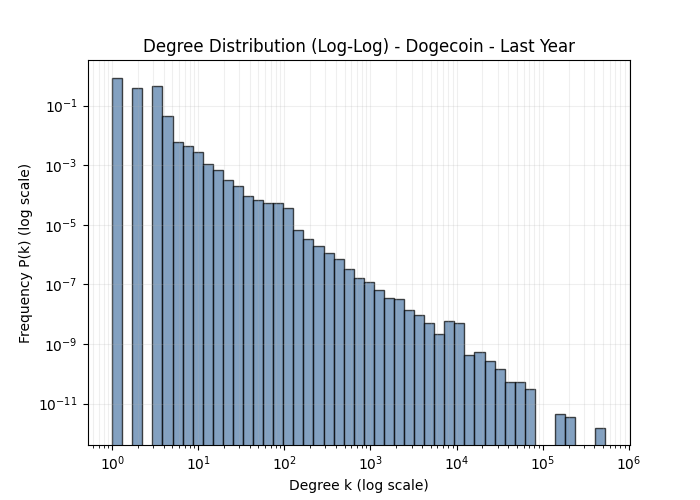
\includegraphics[width=0.65\textwidth]{plots/dogecoin/DegreeDistribution.png}
    \caption{Distribuzione dei gradi $P(k)$ in scala log-log per il network di Dogecoin.}
    \label{fig:doge_degree}
\end{figure}
La Figura~\ref{fig:doge_degree} mostra una decadenza log-log di forma scale-free, ma con due differenze sostanziali rispetto alle altre reti. In primo luogo, la coda si estende solo fino a $k \approx 10^5$ (un ordine di grandezza inferiore rispetto a Bitcoin ed Ethereum), riflettendo la dimensione complessivamente più ridotta del network. In secondo luogo, le tre curve (\texttt{channels $\ge$ 2}, \texttt{top10 removed}, \texttt{top100 removed}) mostrano una sovrapposizione quasi perfetta per $k < 10$, indicando che la parte bassa della distribuzione è identica indipendentemente dalla presenza degli hub, mentre le divergenze si concentrano sui gradi più alti.

\subsubsection{Average Neighbor Degree ($AND$)}
\begin{figure}[H]
    \centering
    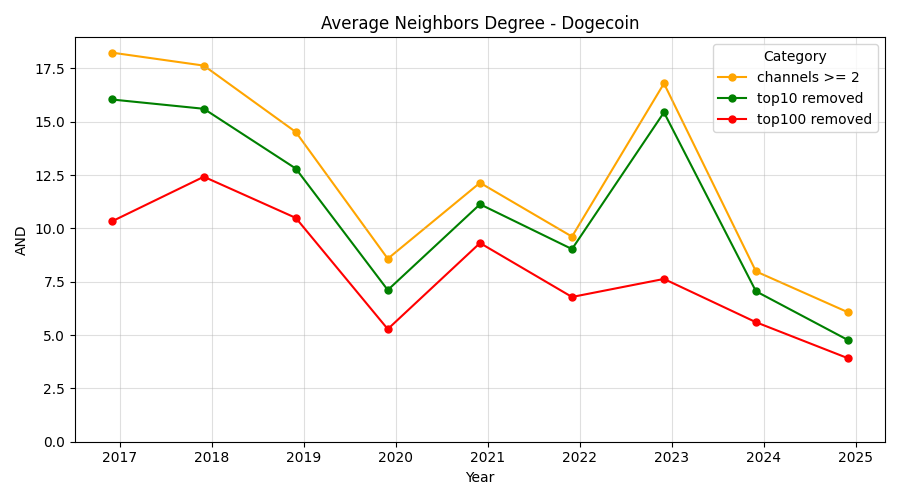
\includegraphics[width=0.65\textwidth]{plots/dogecoin/AverageNeighborsDegree.png}
    \caption{Andamento storico dell'Average Neighbor Degree (AND) in Dogecoin.}
    \label{fig:doge_and}
\end{figure}
L'AND di Dogecoin (Figura~\ref{fig:doge_and}) presenta il valore di partenza più elevato del pannello: $\sim$18.3 nel 2017. Scende poi gradualmente, con uno spike secondario a $\sim$16.8 nel 2023, e crolla a $\sim$6 nel 2025 (ultimo snapshot disponibile). Si nota che i dati si fermano al 2025: i dataset pubblici di Dogecoin disponibili su BigQuery al momento dell'estrazione non includevano transazioni sufficienti a costruire lo snapshot 2026. Il calo terminale è il più brusco osservato nell'intero pannello e coincide con l'esplosione delle componenti connesse nel 2024--2025, che diluisce la connettività media abbassando drasticamente il grado percepito dai nodi periferici.

\subsubsection{Clustering Coefficient ($CC$) ed Esplosione delle Clique}
\begin{figure}[H]
    \centering
    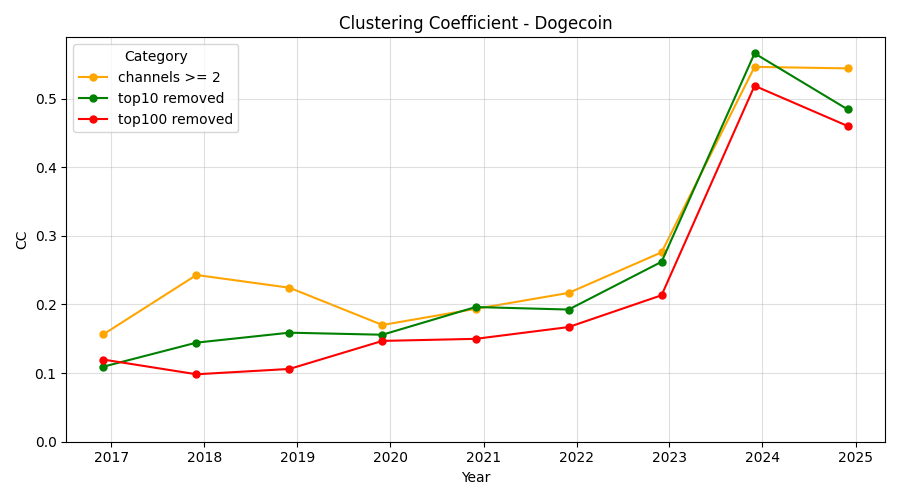
\includegraphics[width=0.65\textwidth]{plots/dogecoin/ClusteringCoefficient.png}
    \caption{Anomala evoluzione del Clustering Coefficient (CC) e saturazione locale in Dogecoin.}
    \label{fig:doge_cc}
\end{figure}
Il CC di Dogecoin (Figura~\ref{fig:doge_cc}) è il dato più anomalo del pannello. Il valore rimane stabile attorno a $\sim$0.25 dal 2017 al 2023, poi subisce nel 2024 un'esplosione senza precedenti: la curva arancione raggiunge $\sim$0.54, la curva verde (\texttt{channels $\ge$ 2, no loops}) supera la curva arancione portandosi a $\sim$0.56, e la curva rossa (\texttt{top100 removed}) sale a $\sim$0.51. Nel 2025 i valori restano elevati ($\sim$0.48--0.52), confermando che l'esplosione del 2024 non è un artefatto transitorio. Questo fenomeno è correlabile con l'esplosione delle componenti connesse nello stesso biennio: l'ingresso massiccio di nuovi nodi che si collegano preferenzialmente agli stessi hub crea strutture a clique dense. Il sorpasso della curva verde (\texttt{no loops}) su quella arancione merita un'osservazione: il leggero scarto tra le due curve potrebbe essere in parte attribuibile alla presenza di self-loop nel grafo e al modo in cui questi interagiscono con il calcolo del CC, piuttosto che riflettere una differenza strutturale reale.

\subsubsection{Network Centralization ($NC$)}
\begin{figure}[H]
    \centering
    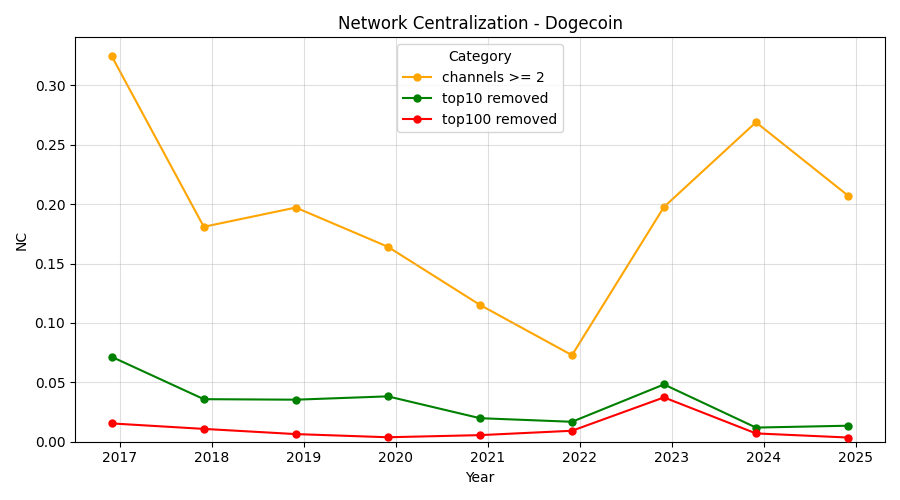
\includegraphics[width=0.65\textwidth]{plots/dogecoin/NetworkCentralization.png}
    \caption{Evoluzione storica dell'indice di Network Centralization (NC) in Dogecoin.}
    \label{fig:doge_nc}
\end{figure}
Il grafico della NC di Dogecoin (Figura~\ref{fig:doge_nc}) mostra il valore iniziale più alto del pannello: $\sim$0.322 nel 2017. La NC scende poi fino al minimo di $\sim$0.072 nel 2022, anno del crollo FTX (visibile nel grafico del prezzo, Figura~\ref{fig:doge_price}), per poi risalire a $\sim$0.267 nel 2024. Questo pattern di ri-centralizzazione nel 2024 è direttamente correlabile con gli eventi elettorali negli USA (novembre 2024) e il relativo interesse speculativo su DOGE, che ha stimolato la costruzione di hub di routing da parte di attori coordinati. Nel 2025 la NC torna a $\sim$0.18, suggerendo un parziale ribilanciamento.

\subsubsection{Componenti Connesse}
\begin{figure}[H]
    \centering
    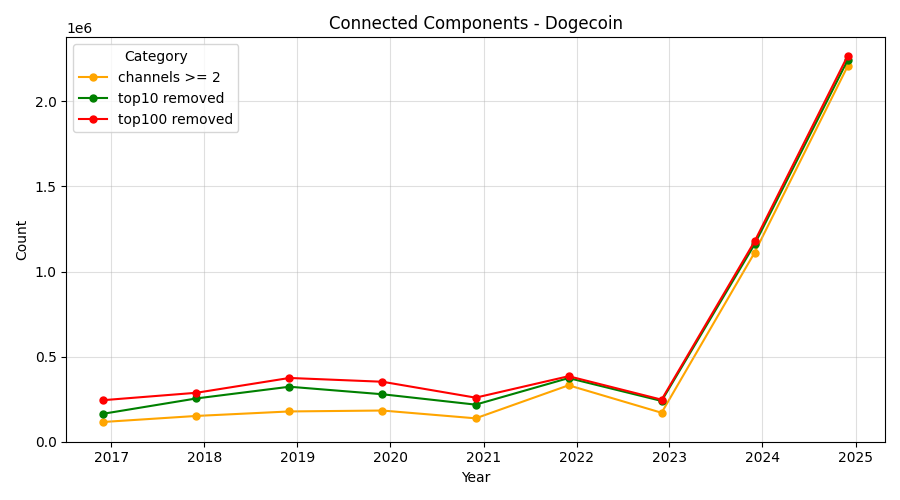
\includegraphics[width=0.65\textwidth]{plots/dogecoin/ConnectedComponents.png}
    \caption{Esplosione delle componenti connesse in Dogecoin (2024--2025).}
    \label{fig:doge_cc_comp}
\end{figure}
Il grafico delle componenti connesse (Figura~\ref{fig:doge_cc_comp}) mostra la dinamica più drammatica del pannello in termini di variazione relativa. Dal 2017 al 2023 il numero di componenti rimane stabile tra 170.000 e 380.000, poi nel 2024 esplode a $\sim$1.1 milioni e nel 2025 raddoppia ulteriormente a $\sim$2.2 milioni. Tutte e tre le curve crescono pressoché parallelamente, indicando che la frammentazione è un fenomeno distribuito non imputabile ai soli hub. Questo dato è apparentemente in contraddizione con l'aumento della NC nello stesso periodo: la spiegazione è che nel 2024 entrarono molti nodi nuovi che formavano piccoli cluster locali densi (spiegando l'esplosione del CC) ma non erano connessi al nucleo principale di routing, generando milioni di componenti isolate.

\subsubsection{Betweenness Centrality ($BC$)}
\begin{figure}[H]
    \centering
    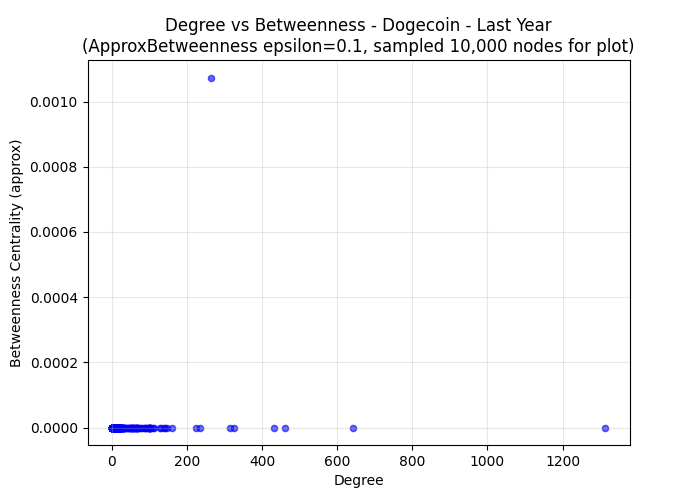
\includegraphics[width=0.65\textwidth]{plots/dogecoin/NodeDegreeBetweennessCentrality.png}
    \caption{Relazione tra Degree e Betweenness Centrality in Dogecoin.}
    \label{fig:doge_bc}
\end{figure}
Il plot Degree-Betweenness di Dogecoin (Figura~\ref{fig:doge_bc}) mostra il grado massimo più basso del pannello ($k \approx 450$), coerente con la dimensione complessivamente più ridotta del network. La distribuzione dei valori di BC è concentrata su pochi nodi ad alto grado, senza bridge node anomali come in Bitcoin. Quasi tutti i nodi con $k < 50$ presentano BC $\approx 0$, confermando che il routing è quasi interamente mediato dagli hub principali.

\subsubsection{Small World Check}
\begin{figure}[H]
    \centering
    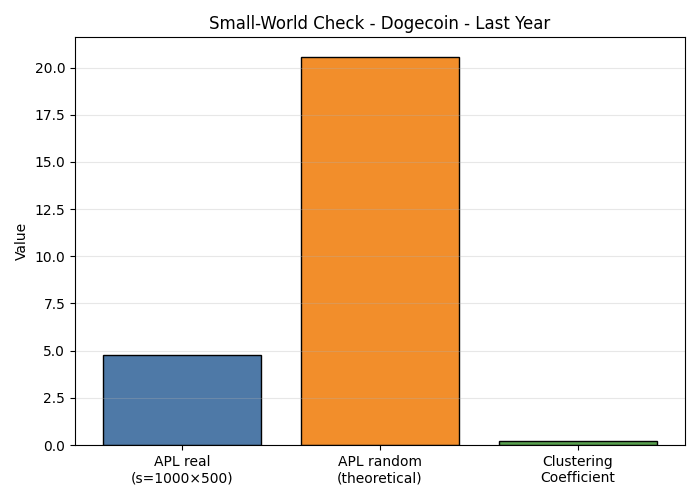
\includegraphics[width=0.65\textwidth]{plots/dogecoin/SmallWorld.png}
    \caption{Grafico di controllo Small World per Dogecoin: APL reale vs.\ modello casuale.}
    \label{fig:doge_sw}
\end{figure}
Il grafico a barre (Figura~\ref{fig:doge_sw}) mostra un APL reale di $\sim$4.7 salti, a fronte di un valore atteso per un grafo casuale di $\sim$20.6. Il rapporto di efficienza ($\sim$4.4$\times$) è paragonabile a Bitcoin. Il Clustering Coefficient riportato nella barra è visibilmente più alto rispetto alle altre reti ($\sim$0.5 dopo il 2024), il che soddisfa la seconda condizione di Watts-Strogatz in misura eccezionale. Tuttavia è importante contestualizzare: un CC così elevato in una rete fortemente centralizzata non indica ridondanza distribuita bensì densità locale attorno a pochi hub, che pur garantendo percorsi brevi non offre la resilienza distribuita tipica dei veri Small World.

\subsection{Conclusioni e Comparazione}
Dogecoin presenta la topologia più anomala del pannello, con dinamiche strutturali nettamente separate in due epoche: pre-2024, caratterizzata da relativa stabilità con 170.000--380.000 componenti e CC $\sim$0.25; e post-2024, con un'esplosione simultanea di componenti connesse (fino a 2.2 milioni), CC ($\sim$0.54) e NC ($\sim$0.267) che segnala l'ingresso massiccio di nuovi nodi organizzati in cluster locali densi ma isolati dal nucleo di routing. Questa biforcazione temporale non ha paralleli nelle altre reti del pannello e sembra correlata agli eventi macroeconomici e politici del 2024, visibili nel grafico del prezzo (Figura~\ref{fig:doge_price}). La dimensione assoluta del network rimane significativamente inferiore alle altre reti: il grado massimo osservato è $k \approx 450$, contro $k \approx 10^6$ di Bitcoin. Questo limite strutturale riduce la capacità di routing su scala globale nonostante l'APL favorevole.

\newpage

\section{Discussione e Comparazione dei Risultati}
L'integrazione sistematica delle metriche analizzate e la discussione approfondita dei rispettivi plot permettono di delineare un quadro matematico chiaro, evidenziando un profondo paradosso strutturale che caratterizza l'evoluzione delle soluzioni di secondo livello. I dati raccolti dimostrano empiricamente che le reti operanti tramite canali di pagamento tendono a evolvere spontaneamente verso strutture con proprietà \textit{scale-free} e \textit{small-world}.

Se da un lato questa conformazione geometrica garantisce un'eccellente efficienza nell'instradamento dei flussi economici, riducendo l'Average Path Length a pochissimi salti medi, dall'altro lato tale efficienza risulta interamente dipendente dalla centralizzazione della liquidità e del capitale attorno a una ristrettissima cerchia di hub dominanti. Come evidenziato dai crolli dell'indice di Network Centralization e dalla frammentazione osservata nei grafici delle Componenti Connesse all'esclusione dei primi 100 nodi, la stabilità e l'esistenza stessa del tessuto transazionale periferico dipendono in modo causale dall'intermediazione di questi grandi poli centrali.

Questo fenomeno non deve essere interpretato come un errore di progettazione del software, bensì costituisce una conseguenza deterministica derivante dalle dinamiche di \textit{preferential attachment} (collegamento preferenziale) e dagli incentivi economici nativi del protocollo. Poiché i nodi che instradano con successo i pagamenti accumulano fee transazionali e incrementano la propria capacità di liquidità, i nuovi partecipanti al network trovano economicamente più conveniente ed efficiente aprire canali con hub già capillarmente interconnessi, amplificando la concentrazione esistente.

\begin{table}[htbp]
\centering
\small
\begin{tabular}{@{}lcccc@{}}
\toprule
Metrica & Bitcoin & Ethereum & Litecoin & Dogecoin \\
\midrule
AND massimo osservato & $\sim$16.5 & $\sim$15.3 & $\sim$19.3 & $\sim$18.3 \\
CC massimo osservato & $\sim$0.21 & $\sim$0.31 & $\sim$0.20 & $\sim$0.54 \\
NC media & $\sim$0.12 & $\sim$0.29 & $\sim$0.18 & $\sim$0.20 \\
APL reale & $\sim$5.35 & $\sim$4.3 & $\sim$4.5 & $\sim$4.7 \\
APL grafo casuale & $\sim$24.0 & $\sim$24.8 & $\sim$14.0 & $\sim$20.6 \\
Rapporto APL & $4.5\times$ & $5.8\times$ & $3.1\times$ & $4.4\times$ \\
Componenti connesse (picco) & $\sim$4.2\,M & $\sim$4.0\,M & $\sim$3.4\,M & $\sim$2.2\,M \\
Grado massimo osservato & $\sim$$10^6$ & $\sim$1750 & $\sim$$10^6$ & $\sim$450 \\
\bottomrule
\end{tabular}
\caption{Confronto dei valori caratteristici delle principali metriche topologiche per i quattro network analizzati. Per Bitcoin, il picco delle componenti connesse si riferisce al grafo con i 100 nodi principali rimossi (\texttt{top100 removed}); per gli altri network le tre varianti di grafo producono valori analoghi.}
\label{tab:comparazione}
\end{table}

La Tabella~\ref{tab:comparazione} sintetizza i valori caratteristici delle metriche principali per i quattro network. La comparazione mette in luce tre profili architetturali distinti. Bitcoin e Litecoin, condividendo la medesima architettura UTXO con SegWit e la stessa implementazione Lightning Network, mostrano distribuzioni di gradi quasi identiche (coda fino a $k \approx 10^6$) e APL reali comparabili. Le differenze emergono nella Network Centralization media: Litecoin registra valori leggermente più alti di Bitcoin ($\sim$0.18 contro $\sim$0.12), spiegabili con la minore numerosità assoluta del network, che amplifica il peso proporzionale dei top hub. Ethereum si distingue per la NC strutturalmente più alta del pannello, pari a $\sim$0.29, e per la dimensione orizzontale più contenuta: il grado massimo osservato è $k \approx 1750$, quattro ordini di grandezza inferiore a Bitcoin. L'APL più basso dell'intero pannello, $\sim$4.3 salti, completa il quadro. Questi tre indicatori sono coerenti con una rete dominata da pochissimi operatori che accorciano i percorsi medi a scapito della ridondanza strutturale. Dogecoin costituisce una categoria a sé, con un Clustering Coefficient post-2024 ($\sim$0.54) senza paralleli nel pannello e un grado massimo di soli $k \approx 450$, riflettendo una rete ancora in fase sperimentale priva di una base consolidata di operatori di routing.

Dal punto di vista delle dinamiche temporali, tutti e quattro i network mostrano correlazioni rilevanti tra gli eventi macroeconomici osservati nei rispettivi grafici di prezzo e le variazioni delle metriche topologiche. Gli anni immediatamente successivi ai massimi storici (2018 per Bitcoin ed Ethereum, 2022 per tutti i network dopo il crollo dell'exchange FTX) mostrano sistematicamente un incremento della Network Centralization: al deflusso dei nodi periferici speculativi il grafo residuo è composto in misura crescente da hub di routing professionali, che acquisiscono maggiore peso strutturale proporzionale. Viceversa, le fasi di bull market (2020--2021 per tutti i network, 2024 per Dogecoin) tendono a produrre un aumento del Clustering Coefficient, poiché i nuovi nodi si collegano preferenzialmente agli stessi hub centrali, generando triangoli locali densi. Il meccanismo di preferential attachment si intensifica dunque proprio nelle fasi di espansione rapida, quando i nuovi partecipanti, privi di infrastruttura consolidata, si affidano agli operatori già visibili e liquidi.

Un aspetto di rilievo pratico riguarda le implicazioni in termini di resilienza alla censura. Una rete hub-and-spoke è strutturalmente vulnerabile ad attacchi mirati ai nodi centrali: la rimozione dei soli 100 hub principali, documentata nei rispettivi grafici delle Componenti Connesse, provoca la dissoluzione del nucleo di routing e l'isolamento dei nodi periferici. Questo dato contrasta con l'obiettivo originario di un sistema di pagamento \textit{censorship-resistant}: un avversario in grado di compromettere o coercire un numero limitato di operatori potrebbe di fatto interrompere il routing per una quota significativa della rete. La resilienza effettiva non è pertanto proporzionale alla dimensione totale del network, ma alla distribuzione della connettività tra i nodi più critici.

In conclusione, la Lightning Network e i protocolli adiacenti manifestano una tendenza evolutiva a replicare autonomamente le medesime strutture fortemente polarizzate di tipo \textit{hub-and-spoke} che caratterizzano i circuiti di pagamento tradizionali come Visa o Mastercard. Il superamento del trilemma della blockchain a livello Layer 2 introduce pertanto un trade-off di natura politica ed economica: l'ottenimento della scalabilità transazionale globale e l'abbattimento delle fee avvengono a spese di una parziale rinuncia alla decentralizzazione strutturale originaria, riproponendo la necessità di figure di intermediazione finanziaria all'interno di sistemi nati per essere nativamente \textit{peer-to-peer}.

\newpage

\section{Conclusioni}

Il presente elaborato ha analizzato l'evoluzione topologica di quattro reti di canali di pagamento Layer 2 (Bitcoin, Ethereum, Litecoin e Dogecoin) attraverso sette metriche strutturali calcolate su snapshot annuali nel periodo 2017--2026 (2017--2025 per Dogecoin). I risultati ottenuti permettono di rispondere in modo netto alla domanda di ricerca centrale: le reti di pagamento off-chain, pur essendo state concepite con l'obiettivo esplicito di replicare il modello peer-to-peer originario della blockchain, convergono spontaneamente verso topologie di tipo \textit{hub-and-spoke} strutturalmente analoghe ai sistemi di pagamento tradizionali che intendevano sostituire.

Tutti e quattro i network analizzati presentano una distribuzione dei gradi conforme a una legge di potenza, confermando la natura \textit{scale-free} delle reti. La proprietà \textit{small-world} è verificata in tutti i casi in cui i dati lo consentono: l'Average Path Length reale risulta sistematicamente inferiore di un ordine di grandezza rispetto alla stima teorica per un grafo casuale di pari dimensioni, garantendo un'efficienza di routing eccezionale. Tuttavia, questa efficienza si rivela strutturalmente dipendente dalla presenza di un ristretto nucleo di hub dominanti: la rimozione dei soli 100 nodi a grado più elevato provoca un crollo immediato dell'indice di Network Centralization verso valori prossimi allo zero e un incremento significativo delle componenti disconnesse, dimostrando che la periferia della rete non possiede alcuna autonomia topologica al di fuori dell'intermediazione degli hub centrali.

I quattro network mostrano traiettorie storiche differenziate. Bitcoin presenta la rete più matura e liquida, con cicli di centralizzazione correlati agli halving quadriennali. Ethereum, pur esibendo l'Average Path Length più basso del gruppo, indicatore della massima efficienza di routing, ha visto la propria infrastruttura di canali puri progressivamente marginalizzata a vantaggio dei sistemi Rollup, che offrono scalabilità senza richiedere apertura esplicita di canali bilaterali. Litecoin mostra la traiettoria più lineare e stabile, replicando la struttura topologica di Bitcoin grazie alla medesima architettura UTXO, con barriere di ingresso più basse che favoriscono una crescita organica e progressiva. Dogecoin rappresenta il caso limite dell'intero paniere: l'esplosione del Clustering Coefficient nel 2024, con valori che raggiungono $\sim$0.55, segnala la formazione di strutture quasi-clique tra i nodi centrali, indicando un processo di ultra-centralizzazione che riduce la rete off-chain a un oligopolio di pochi operatori industriali.

\paragraph{Limiti dello studio.} La metodologia adottata presenta alcune limitazioni che è opportuno esplicitare. Il pre-filtraggio con la condizione $\text{edge} \ge 2$, reso necessario dai vincoli hardware descritti nel Capitolo~2, esclude per costruzione la componente più volatile e periferica della rete, determinando una sottostima del numero reale di partecipanti e una sovrastima del grado di connettività media. L'analisi è inoltre condotta su grafi non pesati, prescindendo dalla capacità di liquidità allocata nei singoli canali: due reti con topologia identica possono differire radicalmente nella loro efficienza economica reale se la distribuzione della liquidità è asimmetrica. Infine, l'approssimazione stocastica della Betweenness Centrality e il campionamento bidirezionale dell'APL introducono un errore controllato ma non nullo, che potrebbe influenzare le stime su grafi di dimensioni particolarmente ridotte come quello di Dogecoin.

\paragraph{Sviluppi futuri.} Le limitazioni identificate aprono direzioni di ricerca complementari. Un'estensione naturale del presente lavoro è l'analisi dei grafi \textit{pesati} per capacità di liquidità, che consentirebbe di distinguere la centralità topologica dalla centralità economica e di valutare la resilienza della rete in termini di flusso massimo piuttosto che di connettività strutturale. Un secondo sviluppo di interesse riguarda l'adozione di modelli di grafo \textit{dinamici} in sostituzione degli snapshot statici annuali, per catturare le transizioni di fase topologiche in corrispondenza degli eventi macroeconomici chiave. Infine, l'estensione dell'analisi ad altri network emergenti (come la rete di canali di Ark Protocol o le implementazioni Lightning su altcoin minori) permetterebbe di verificare la generalità delle tendenze osservate e di stabilire se la convergenza verso strutture hub-and-spoke costituisca una proprietà universale dei sistemi di pagamento off-chain o un artefatto specifico dei protocolli analizzati.

\newpage
\printbibliography

\end{document}
